\documentclass[
  paper=a4,
  % version=3.25,
  pagesize=pdftex,
  twoside=false,
  toc=listof,
  BCOR=0pt,
  DIV=15,
  indent,
]{scrartcl}
\usepackage{ctex}
\usepackage{tcolorbox}
\usepackage{pdfpages}
\usepackage{tikz-network}
\usepackage{tikz-network-documentation}


\newcommand{\MS}{Martin Scheidt}

\hypersetup{
  pdftitle={tikz/networkmanual},
  pdfsubject={A tikz toolbox for track schematics},
  pdfauthor={Latex Studio},
  pdfkeywords={latex, tikz, library, railway, track, layout}
}


\begin{document}

% \includepdf[pages={1}]{Template_5fengmian.pdf}

% \newpage

\title{\tikz\node[scale=1.2]{\color{gray}\Huge\sffamily \{\textcolor{black}{Ti\textcolor{orange}{\emph{k}}Z}-\textcolor{blue}{networkmanual}\}};}
\subtitle{Ti\emph{k}Z \textcolor{orange}{\&} PGF \textcolor{blue}{神经网络图形绘制}}
\author{\vhListAllAuthorsLong}
\date{Version \vhCurrentVersion~ from \vhCurrentDate}

\maketitle
\thispagestyle{empty}
\begin{multicols}{2}
  \tableofcontents
\end{multicols}
\vspace{1.5cm}
\begin{multicols}{2}
\centerline{
  \begin{tikzpicture}[multilayer=3d,scale=1.3]
    \Plane[x=-.5,y=-.5,width=3,height=2.5]
    \Plane[x=1.7,y=-3.5,width=3,height=2.5,grid=5mm]
    \Vertices{mlvertices.csv}
    \Edges{mledges.csv}
    \end{tikzpicture}
}


  \centerline{
    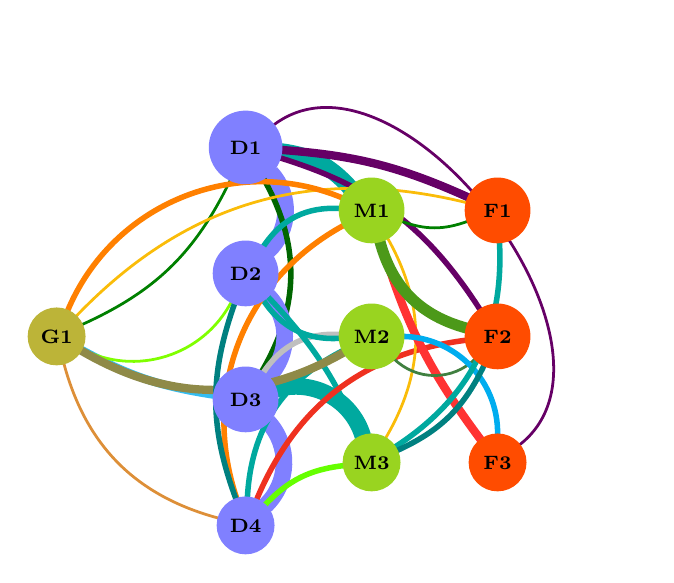
\begin{tikzpicture}[scale=0.8]
    %\draw (-4,-4)grid (6,4);
      \Vertex[x=-3,y=0,style={color=yellow!70!black},size=0.7,label=\bfseries G1]{G1}
      \Vertex[x=0,y=3,style={color=blue!50!white},label=\bfseries D1,size=0.9]{D1}
      \Vertex[x=0,y=1,style={color=blue!50!white},label=\bfseries D2,size=0.8]{D2}
      \Vertex[x=0,y=-1,style={color=blue!50!white},label=\bfseries D3,size=0.8]{D3}
      \Vertex[x=0,y=-3,style={color=blue!50!white},label=\bfseries D4,size=0.7]{D4}
      \Vertex[x=2,y=2,style={color=yellow!60!green},label=\bfseries M1,size=0.8]{M1}
      \Vertex[x=2,y=0,style={color=yellow!60!green},label=\bfseries M2,size=0.8]{M2}
      \Vertex[x=2,y=-2,style={color=yellow!60!green},label=\bfseries M3,size=0.7]{M3}
      \Vertex[x=4,y=2,style={color=orange!60!red},label=\bfseries F1,size=0.8]{F1}
      \Vertex[x=4,y=0,style={color=orange!60!red},label=\bfseries F2,size=0.8]{F2}
      \Vertex[x=4,y=-2,style={color=orange!60!red},label=\bfseries F3,size=0.7]{F3}
      % Edges D
      \Edge[bend=45,color=blue!50!white,lw=6pt](D1)(D2)
      \Edge[bend=30,color=black!60!green,lw=2pt](D1)(D3)
      \Edge[bend=45,color=blue!50!white,lw=6pt](D2)(D3)
      \Edge[bend=45,color=blue!50!white,lw=6pt](D3)(D4)
      \Edge[bend=45,color=cyan!50!green,lw=6pt](D3)(M3)
      \Edge[bend=30,color=gray!50!white,lw=2pt](D3)(M2)
      \Edge[bend=20,color=cyan!50!green,lw=6pt](D1)(M1)
      \Edge[bend=10,color=violet!80!black,lw=3pt](D1)(F1)
      \Edge[bend=20,color=violet!80!black,lw=2pt](D1)(F2)
      \Edge[bend=90,color=violet!80!black,lw=1pt](D1)(F3)
      \Edge[bend=30,color=cyan!50!green,lw=2pt](D2)(M1)
      \Edge[bend=-30,color=cyan!50!green,lw=2pt](D2)(M2)
      \Edge[bend=10,color=cyan!50!green,lw=2pt](D2)(M3)
      \Edge[bend=40,color=orange,lw=2pt](D4)(M1)
      \Edge[bend=30,color=cyan!50!green,lw=2pt](D4)(M2)
      \Edge[bend=30,color=yellow!10!red,lw=2pt](D4)(F2)
      % Edges G1
      \Edge[bend=-20,color=black!50!green,lw=1pt](G1)(D1)
      \Edge[bend=30,color=yellow!50!orange,lw=1pt](G1)(F1)
      \Edge[bend=-30,color=yellow!50!purple,lw=1pt](G1)(D4)
      \Edge[bend=-10,color=cyan!80!white,lw=3pt](G1)(D3)
      \Edge[bend=-45,color=green!50!yellow,lw=1pt](G1)(D2)
      \Edge[bend=45,color=orange,lw=2pt](G1)(M1)
      \Edge[bend=-30,color=black!50!yellow,lw=3pt](G1)(M2)
      \Edge[bend=-20,color=blue!50!green,lw=2pt](D2)(D4)
      \Edge[bend=20,color=green!60!yellow,lw=2pt](D4)(M3)
      % Edages M
      \Edge[bend=-20,color=black!50!green,lw=1pt](M1)(F1)
      \Edge[bend=30,color=yellow!50!orange,lw=1pt](M1)(M3)
      \Edge[bend=-10,color=red!80!white,lw=3pt](M1)(F3)
      \Edge[bend=-30,color=purple!40!green,lw=4pt](M1)(F2)
      \Edge[bend=-45,color=green!50!violet,lw=1pt](M2)(F2)
      \Edge[bend=45,color=cyan,lw=2pt](M2)(F3)
      \Edge[bend=-30,color=cyan!50!green,lw=2pt](M3)(F1)
      \Edge[bend=-20,color=blue!50!green,lw=2pt](M3)(F2)
    \end{tikzpicture}
  }
  \end{multicols}
\cleardoublepage

\section{序言}\label{sec:intro}

近年来,神经网络学习在越来越多的科学领域得盛行,除了一些实体的理论知识基础之外,视觉的网络位置将复杂的多元关系传达给观众得到越来越多人的广泛使用,使用可视化工具,
有助于结构,过滤,操作,当然也有助于视觉化网络化。但是,它们有一些限制,包括对特定软件工具的需求,嵌入困难将其正确输出到 \LaTeX{} 文件中(例如,字体类型,字体大小,附加
所需的国家方程式和数学符号,...)和挑战图形的后处理,而无需重新运行软件再次使用工具。
为了克服这个问题,软件包 \textcolor{black}{Ti\textcolor{orange}{\emph{k}}Z}-\textcolor{blue}{network}
创建。一些功能是:
\begin{itemize}
  \item \LaTeX{}是科学出版物的标准,被广泛使用
  \item 除了\LaTeX{} 以外,不需要其他软件
  \item 不需要编程技巧
  \item 使用简单,但可以100\% 控制输出
  \item 易于后处理(例如,添加图纸,文本,等,...)
  \item 与文档中相同的字体,字体大小,数学符号...精神
  \item pdf格式不会导致输出质量下降
  \item 网络易于调整或修改以用于讲座或小型考试
  \item 能够可视化更大的网络
  \item (多层)网络的三维可视化
  \item 与其他可视化工具兼容
\end{itemize}

\subsection{如何利用好学习手册(How to read this manual)}
本手册的目的是描述 \textcolor{black}{Ti\textcolor{orange}{\emph{k}}Z} 在可视化网络的使用
用。 为确保易于使用及使内容更加清晰,本手册的结构如下:
\begin{itemize}
\item 在第2章中,创建简单网络的要素(手工)
在飞机上进行了解释。 从而,命令的使用
显示 \verb|\Vertex| 和 \verb|\Edge|。
\item 如何从外部文件1创建复杂的网络
1例如
<grap>或\textcolor{black}{Ti\textcolor{orange}{\emph{k}}Z}-\textcolor{blue}{network}
在第3章中有详细介绍。因此,主要命令为 \verb|\Vertices|
和 \verb|\Edges| 使用,以及相同或者类似可选参数设置元件。
\item 在第4章中,介绍多层次的网络可视化,例如 \verb|\Plane| 和 Layer介绍。
\item 介绍网络图形绘制使用的默认设置以及如何修改它们。
\item 有关故障排除和支持的信息。
\item 由于这是软件包的 Alpha 版本(0.1),因此具有这可能会被添加,并且命令必须固定在附录B中列出。
\end{itemize}

\subsubsection{部分解释(A few explanations)}
本手册中的图像是使用\textcolor{black}{Ti\textcolor{orange}{\emph{k}}Z}-\textcolor{blue}{network} library或Ti\emph{k}Z。 为每个图像指定用于此的代码。

\begin{minipage}[c]{0.51\textwidth}
  \centering
  \begin{lstlisting}[gobble=8]
        
\begin{tikzpicture}
         \filldraw (-.2,.2) circle (2pt)
          (.2,.2) circle (2pt);
         \draw (0,0) circle (5mm) (-.3,-.1) .. controls (0,-.3) ..(.3,-.1);
        \end{tikzpicture}
  \end{lstlisting}
\end{minipage}
\hfil
\begin{minipage}[c]{0.45\textwidth}
  \centering
  
\begin{tikzpicture}
    \filldraw (-.2,.2) circle (2pt) (.2,.2) circle (2pt);
    \draw (0,0) circle (5mm) (-.3,-.1) .. controls (0,-.3) ..
    (.3,-.1);
    \end{tikzpicture}
\end{minipage}

需要特殊添加以更好地理解以橙色显示,但不在可用的示例代码中。

\begin{minipage}[c]{0.51\textwidth}
  \centering
  \begin{lstlisting}[gobble=8]
        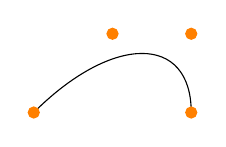
\begin{tikzpicture}
         \draw (0,0) .. controls (1,1) and (2,1) .. (2,0);
         \filldraw[orange](0,0) circle (2pt) (1,1) circle (2pt)(2,1) circle (2pt) (2,0) circle (2pt);
        \end{tikzpicture}
  \end{lstlisting}
\end{minipage}
\hfil
\begin{minipage}[c]{0.45\textwidth}
  \centering
  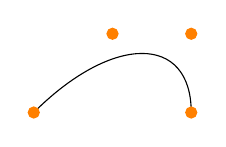
\begin{tikzpicture}
    \draw (0,0) .. controls (1,1) and (2,1) .. (2,0);
    \filldraw[orange](0,0) circle (2pt) (1,1) circle (2pt)(2,1) circle (2pt) (2,0) circle (2pt);
    \end{tikzpicture}
\end{minipage}

  \subsubsection{绘制网图代码输入(Input)}
  \textcolor{black}{Ti\textcolor{orange}{\emph{k}}Z}-网络库中的命令(例如 \verb|\Vertex|,
  \verb|\Edge|)
  始终以大写字母开头,在最后不需要分号 “;”。 布尔参数也以大写字母开头(例如\verb|<NoLabel>|)。 需要用户输入,使用的参数写在小写字母(例如h颜色i)。

基本上,可以区分强制性论点\{\}和可选参数[]。 必须输入第一个值。 相比之下,不需要为可选内容输入任何内容输入。 输入以下内容时,可以激活其他功能(例如\verb|<size>|)
可选参数。输入尺寸值时,基本单位始终是厘米,但在定义线宽等中以pt 为单位。 默认单位可以用\verb|\SetDefaultUnit| 来进行修改; 参见第 5.1 节年龄值 \% 始终指定为十进制值; 例如,100\%= 1.0,而10%对应于0.1。

\subsubsection{下载与安装(Installation)}

实际上,各种软件的安装我们不需要在这里进行赘述,在我们进行安装 \LaTeX{} 时就已经自动有
基本软件包 \textcolor{black}{Ti\textcolor{orange}{\emph{k}}Z}-\textcolor{blue}{network},它是你安装软件的时候就下载好的,它就储存在下载安装的 Texlive 中。另外,该软件包的当前版本可通过 CTAN4 获得。 一种
 4 https://ctan.org/pkg/tikz-network 可获得 \textcolor{black}{Ti\textcolor{orange}{\emph{k}}Z}-\textcolor{blue}{network}下一版本的候选版本
在 github~5 上 5 https://github.com/hackl/
是否安装了软件包或样式文件存储在文件夹中
主文件,因此可以导入库,如下所示示例显示:

\begin{lstlisting}
  % 进行可视化文档的编写 ===============================
  % header 文档的头部主要是文档类型以及导言区导入的宏包或者通过人工手动来进行的设置。
  \documentclass{scrreprt} % 文档类型
  % 导入宏包 packages ---------------------------------
  \usepackage{tikz-network}
  \begin{document}
    % -------------------------------------------------
    文档的其他内容
    % -------------------------------------------------
    % 文档的绘图部分
    \begin{tikzpicture}
      \Vert...
    \end{tikzpicture}
  \end{document}
\end{lstlisting}

\subsection{需要额外添加的宏包(Additional necessary packages)}

要使用 \textcolor{black}{Ti\textcolor{orange}{\emph{k}}Z} 的所有命令和选项,可能需要一些包装
需要重新加载。 这些丢失的文件(或其名称)显示在
转换文件时的错误日志。 但是,对于包装
如本手册中所述,使用库和
\textcolor{black}{Ti\textcolor{orange}{\emph{k}}Z} 标准命令。

\section{简单网图绘制(Simple Networks)}

\subsection{顶点的绘制/输入(Vertex)}

\verb|\Vertex|是基本命令,它可以将顶点放置在
文档并修改其外观。
\verb|\Vertex| [<本地选项>] {名称}
为了能够放置顶点,非空 <Name> 参数是
需要。 此参数定义了顶点的参考名称,
必须是唯一的。 不允许使用数学符号作为名称
以及没有空格。 名称不应与
用于显示的 <label>; 例如,一个人可能想要
显示 A1,而名称将为 A1。
对于\verb|\Vertex|,以下选项可用:

%tab1
\begin{table}[h!]
  \center
  \renewcommand\arraystretch{0.9}
    \caption{Local options for the
    Vertex command.}
  \begin{tabular}{p{60pt}<{\raggedright}p{40pt}<{\raggedright}p{50pt}<{\raggedright}p{150pt}<{\raggedright}}
\hline\\[-5.5mm]\hline
Option &    Default  &   Type  &   Definition\\
\hline
x &  0 &   measure &  x-coordinate\\
y &  0 &  measure &  y-coordinate\\
size &  \{\}  &  measure  &  diameter of the circle\\
color &  \{\} &   color & fill color of vertex\\
opacity &  \{\} &   number &  opacity of the fill color\\
shape &  \{\} &vstring &  shape of the vertex\\
label &  \{\} &   string &  label\\
fontsize &  \{\}  &  string &  font size of the label\\
fontcolor &  \{\} &   color &   font color of the label\\
fontscale &  \{\} &   number &   scale of the label\\
position &  center &   value &   a label position\\
distance &  0 &   measure &   label distance from the center\\
style &  \{\}  &  string &   additional\textcolor{black}{Ti\textcolor{orange}{\emph{k}}Z} styles\\
layer &  \{\}  &  number &   assigned layer of the vertex\\
\hline
NoLabel &  false &  Boolea &  n delete the label\\
IdAsLabel &  false &  Boolean &   uses the Name as label\\
Math &  false &  Boolean &   displays the label in math mode\\
RGB &  false &   Boolean &   allow RGB colors\\
Pseudo &  false &  Boolean &   create a pseudo vertex\\
\hline\\[-5.5mm]\hline
\multicolumn{4}{c}{either measure or string}
  \end{tabular}

\end{table}

选项输入的顺序无关紧要。 变化
可以使用 \verb|\SetVertexStyle|设置为默认的Vertex布局

\verb|\Vertex[<x>=measure, <y>=measure]{Name}|

顶点的位置由笛卡尔坐标确定。
分别在\verb|<x>| 和\verb|<y>|中。 坐标是可选的。 如果没有坐标
确定顶点将放置在原点(0,0)。 环境保护措施以默认单位(厘米)为单位。 更改单位(本地
可通过将单位添加到小节2来完成。 更改为
2 例如 x=1 英寸
可以使用 \verb|\SetDefaultUnit| 进行默认设置;
\begin{verbatim}
  \SetCoordinates[<xAngle>=number,<yAngle>=number, <zAngle>=number,
  <xLength>=number,<yLength>=number,<zLength>=number]
\end{verbatim}

 \begin{minipage}[c]{0.55\textwidth}
   \centering
   \begin{lstlisting}[gobble=8]
        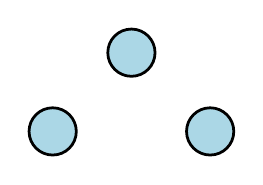
\begin{tikzpicture}
         \Vertex{A}          % 默认的坐标在原点 (0,0)
         \Vertex[x=1,y=1]{B} % 确定了坐标 (1,1)
         \Vertex[x=2]{C}     % 确定了坐标在 (2,0)
        \end{tikzpicture}
   \end{lstlisting}
 \end{minipage}
 \hfil
 \begin{minipage}[c]{0.40\textwidth}
   \centering
   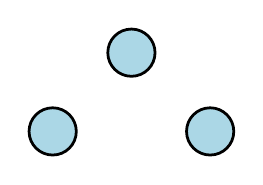
\begin{tikzpicture}
     \Vertex{A}
     \Vertex[x=1,y=1]{B}
     \Vertex[x=2]{C}
     \end{tikzpicture}
 \end{minipage}

\verb|\Vertex[<size>=measure]{Nam}|

顶点的直径可以通过选项 \verb|<size>| 来更改。
默认情况下,顶点的直径为 0.6 厘米。 另外,这里默认
单位为厘米,不必添加到度量中。

\begin{minipage}[c]{0.55\textwidth}
  \centering
  \begin{lstlisting}[gobble=8]
        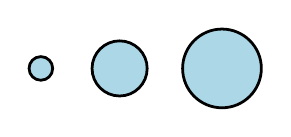
\begin{tikzpicture}
         \Vertex[size=.3]{A}       % 默认的坐标在原点 (0,0),大小为默认的 0.3 倍
         \Vertex[x=1,size=.7]{B}   % 确定了坐标 (1,1),大小为默认的 0.7 倍
         \Vertex[x=2.3,size=1]{C}  % 确定了坐标 (2.3,0),大小为默认的 (1 倍)
        \end{tikzpicture}
  \end{lstlisting}
\end{minipage}
\hfil
\begin{minipage}[c]{0.40\textwidth}
  \centering
  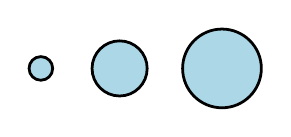
\begin{tikzpicture}
    \Vertex[size=.3]{A}
    \Vertex[x=1,size=.7]{B}
    \Vertex[x=2.3,size=1]{C}
    \end{tikzpicture}
\end{minipage}

\verb|\Vecex[<color>=color]{name}|

要单独更改每个顶点的填充颜色,该选项
我必须使用颜色。 如果没有设置 <RGB> 选项,则默认
可以应用 \textcolor{black}{Ti\textcolor{orange}{\emph{k}}Z} 和 \LaTeX{} 颜色。

\begin{minipage}[c]{0.55\textwidth}
  \centering
  \begin{lstlisting}[gobble=8]
    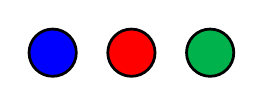
\begin{tikzpicture}
      \Vertex[color = blue]{A}
      \Vertex[x=1,color=red]{B}
      \Vertex[x=2,color=green!70!blue]{C}
    \end{tikzpicture}
  \end{lstlisting}
\end{minipage}
\hfil
\begin{minipage}[c]{0.40\textwidth}
  \centering
  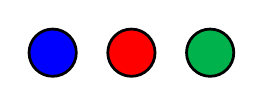
\begin{tikzpicture}
    \Vertex[color = blue]{A}
    \Vertex[x=1,color=red]{B}
    \Vertex[x=2,color=green!70!blue]{C}
    \end{tikzpicture}
\end{minipage}

\verb|\Vecex[<opacity>=number]{name}|

使用选项\verb|<opacity>|,顶点填充颜色的不透明度可以
被修改。 数字范围在 0 到 1 之间。其中 0
代表完全透明的填充,代表 1 的是实心填充。

\begin{minipage}[c]{0.55\textwidth}
  \centering
  \begin{lstlisting}[gobble=8]
       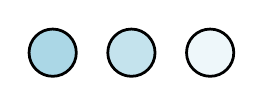
\begin{tikzpicture}
        \Vertex[opacity = 1]{A}
        \Vertex[x=1,opacity =.7]{B}
        \Vertex[x=2,opacity =.2]{C}
       \end{tikzpicture}
  \end{lstlisting}
\end{minipage}
\hfil
\begin{minipage}[c]{0.40\textwidth}
  \centering
  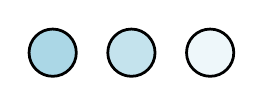
\begin{tikzpicture}
    \Vertex[opacity = 1]{A}
    \Vertex[x=1,opacity =.7]{B}
    \Vertex[x=2,opacity =.2]{C}
    \end{tikzpicture}
\end{minipage}

\verb|\Vecex[<shape>=string]{name}|

使用选项\verb|<shape>|,可以修改顶点的形状。
因此,可以使用在 \textcolor{black}{Ti\textcolor{orange}{\emph{k}}Z}中实现的形状,包括:
圆形,矩形,菱形,梯形,半圆形,等腰三角形,...

\begin{minipage}[c]{0.55\textwidth}
  \centering
  \begin{lstlisting}[gobble=8]
        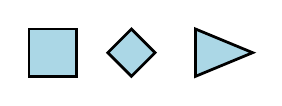
\begin{tikzpicture}
         \Vertex[shape = rectangle]{A}
         \Vertex[x=1,shape = diamond]{B}
         \Vertex[x=2,shape = isosceles triangle]{C}
        \end{tikzpicture}
  \end{lstlisting}
\end{minipage}
\hfil
\begin{minipage}[c]{0.40\textwidth}
  \centering
  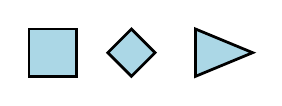
\begin{tikzpicture}
    \Vertex[shape = rectangle]{A}
    \Vertex[x=1,shape = diamond]{B}
    \Vertex[x=2,shape = isosceles triangle]{C}
    \end{tikzpicture}
\end{minipage}

\verb|\Vecex[<label>=string]{name}|

在 \textcolor{black}{Ti\textcolor{orange}{\emph{k}}Z}-\textcolor{blue}{network} 中,有几种方法可以定义标签
顶点和边缘。 常见方法是通过选项\verb|<label>|。
在这里,可以使用任何字符串参数,包括空格的
环境\$ \$可用于显示数学表达式。

\begin{minipage}[c]{0.55\textwidth}
  \centering
  \begin{lstlisting}[gobble=8]
        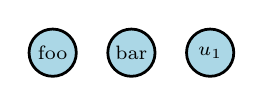
\begin{tikzpicture}
          \Vertex[label=foo]{A}
          \Vertex[x=1,label=bar]{B}
          \Vertex[x=2,label=$u _ 1$]{C}
         \end{tikzpicture}
  \end{lstlisting}
\end{minipage}
\hfil
\begin{minipage}[c]{0.40\textwidth}
  \centering
  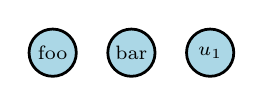
\begin{tikzpicture}
    \Vertex[label=foo]{A}
    \Vertex[x=1,label=bar]{B}
    \Vertex[x=2,label=$u _ 1$]{C}
    \end{tikzpicture}
\end{minipage}

\begin{verbatim}
  \Vecex[<label>=string,<fontsize>=<tiny/scriptsize/footnotesize/
  small/large/Large/huge/...>]{name}
\end{verbatim}

\verb|<label>|的字体大小可以通过以下选项进行修改
\verb|<fontsize>|。 这里可以使用常用的\LaTeX{}字体大小例如
\verb|\tiny,\scriptsize,\footnotesize,\small,...|
更改标签的大小。

\begin{minipage}[c]{0.55\textwidth}
  \centering
  \begin{lstlisting}[gobble=8]
        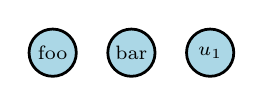
\begin{tikzpicture}
          \Vertex[label=foo]{A}
          \Vertex[x=1,label=bar]{B}
          \Vertex[x=2,label=$u _ 1$]{C}
         \end{tikzpicture}
  \end{lstlisting}
\end{minipage}
\hfil
\begin{minipage}[c]{0.40\textwidth}
  \centering
  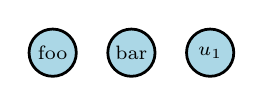
\begin{tikzpicture}
    \Vertex[label=foo]{A}
    \Vertex[x=1,label=bar]{B}
    \Vertex[x=2,label=$u_1$]{C}
    \end{tikzpicture}
\end{minipage}

\verb|\Vecex[<label>=string,<fontcolor>=color]{name}|

% \begin{minipage}[c]{0.55\textwidth}
%   \centering
%   \begin{lstlisting}[gobble=8]
%         \begin{tikzpicture}
%           \Vertex[label=foo]{A}
%           \Vertex[x=1,label=bar]{B}
%           \Vertex[x=2,label=$u _ 1$]{C}
%          \end{tikzpicture}
%   \end{lstlisting}
% \end{minipage}
% \hfil
% \begin{minipage}[c]{0.40\textwidth}
%   \centering
%   \begin{tikzpicture}
%     \Vertex[label=foo]{A}
%     \Vertex[x=1,label=bar]{B}
%     \Vertex[x=2,label=$u_1$]{C}
%     \end{tikzpicture}
% \end{minipage}

\verb|<lable>|的颜色可以使用选项\verb|<fontcolor>|进行更改。当前,仅支持默认的TikZ和\LaTeX{}颜色。

\begin{minipage}[c]{0.55\textwidth}
  \centering
  \begin{lstlisting}[gobble=8]
        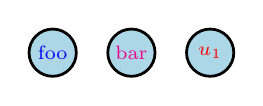
\begin{tikzpicture}
         \Vertex[label=foo,fontcolor=blue]{A}
         \Vertex[x=1,label=bar,fontcolor=magenta]{B}
         \Vertex[x=2,label=$u _ 1$,fontcolor=red]{C}
        \end{tikzpicture}
  \end{lstlisting}
\end{minipage}
\hfil
\begin{minipage}[c]{0.40\textwidth}
  \centering
  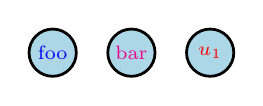
\begin{tikzpicture}
    \Vertex[label=foo,fontcolor=blue]{A}
    \Vertex[x=1,label=bar,fontcolor=magenta]{B}
    \Vertex[x=2,label=$u _ 1$,fontcolor=red]{C}
    \end{tikzpicture}
\end{minipage}

\verb|\Vecex[<label>=string,<fontscale>=number]{name}|
与选项~\verb|<fontsize>| 相反,选项~\verb|<fontscale>|
本身不会更改字体大小,但会放大当前字体大小
或下降。 数字定义比例,其中
0 和 1 向下缩放字体和数字,大于1向上缩放
标签。 例如~0.5 将字体的大小减小到其字体的 50\%
原始大小,而 1.2 会将字体缩放为 120\%。

\begin{minipage}[c]{0.55\textwidth}
  \centering
  \begin{lstlisting}[gobble=8]
        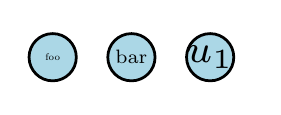
\begin{tikzpicture}
          \Vertex[label=foo,fontscale=0.5]{A}
          \Vertex[x=1,label=bar,fontscale=1]{B}
          \Vertex[x=2,label=$u _ 1$,fontscale=2]{C}
        \end{tikzpicture}
  \end{lstlisting}
\end{minipage}
\hfil
\begin{minipage}[c]{0.40\textwidth}
  \centering
  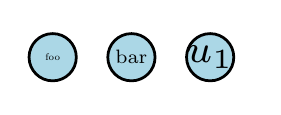
\begin{tikzpicture}
    \Vertex[label=foo,fontscale=0.5]{A}
    \Vertex[x=1,label=bar,fontscale=1]{B}
    \Vertex[x=2,label=$u _ 1$,fontscale=2]{C}
    \end{tikzpicture}
\end{minipage}

\verb|\Vecex[<label>=string,<position>=value,<distance>=number]{name}|

默认情况下,\verb|<laabel>|的\verb|<position>|位于顶点的中心。
特克斯 经典的 \textcolor{black}{Ti\textcolor{orange}{\emph{k}}Z}命令6可用于更改\verb|<label>|位置
例如 上方,下方,左侧,右侧,左侧上方,
在右上方,\verb|<label>|。 相反,使用这样的命令,位置可以是
输入一个介于-360和
360.原点(0◦)是y轴。 正数改变
逆时针旋转我的位置,而负数进行更改
顺时针。

如果选择,则\verb|<distance>|是顶点与顶点之间的距离
标签可以更改。

\begin{minipage}[c]{0.55\textwidth}
  \centering
  \begin{lstlisting}[gobble=8]
        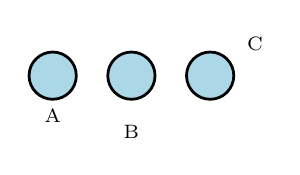
\begin{tikzpicture}
        \Vertex[label=A,position=below]{A}
        \Vertex[x=1,label=B,position=below,distance=2mm]{B}
        \Vertex[x=2,label=C,position=30,
        distance=1mm]{C}
        \end{tikzpicture}
  \end{lstlisting}
\end{minipage}
\hfil
\begin{minipage}[c]{0.40\textwidth}
  \centering
  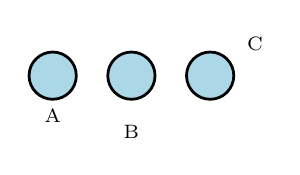
\begin{tikzpicture}
    \Vertex[label=A,position=below]{A}
    \Vertex[x=1,label=B,position=below,distance=2mm]{B}
    \Vertex[x=2,label=C,position=30,distance=1mm]{C}
    \end{tikzpicture}
\end{minipage}

\verb|\Vecex[<style>={string}]{name}|

任何其他 \textcolor{black}{Ti\textcolor{orange}{\emph{k}}Z} 样式选项或命令都可以通过输入
选项\verb|<style>|。 这些命令大多数都可以在
“\textcolor{black}{Ti\textcolor{orange}{\emph{k}}Z}/PGF 手册”。 包含命令可选择
位置(例如\verb|<shading>=ball|),那么我的 <style> 参数必须为
在\{\}个括号之间。

\begin{minipage}[c]{0.55\textwidth}
  \centering
  \begin{lstlisting}[gobble=8]
         
\begin{tikzpicture}
          \Vertex[style={color=red}]{A} % 内部颜色填充
          \Vertex[x=1,style=dashed]{B} % 边缘虚线
          \Vertex[x=2,style={shading=ball}]{C} % 立体颜色填充
         \end{tikzpicture}
  \end{lstlisting}
\end{minipage}
\hfil
\begin{minipage}[c]{0.40\textwidth}
  \centering
  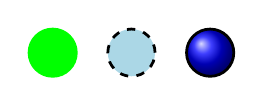
\begin{tikzpicture}
    \Vertex[style={color=green}]{A}
    \Vertex[x=1,style=dashed]{B}
    \Vertex[x=2,style={shading=ball}]{C}
    \end{tikzpicture}
\end{minipage}

\verb|\Vertex<IdAsLabel>]{Name}|

\verb|\Vertex[<NoLabel>,<label>=string]{Name}|

\verb|<IdAsLabel>|是一个布尔选项,用于分配
顶点作为标签。 相反,\verb|\Vertex[<NoLabel>|禁止所有标签。

\begin{minipage}[c]{0.55\textwidth}
  \centering
  \begin{lstlisting}[gobble=8]
        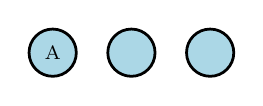
\begin{tikzpicture}
         \Vertex[IdAsLabel]{A} % 分配顶点标签
         \Vertex[x=1,label=B,NoLabel]{B} % 禁止顶点标签
         \Vertex[x=2,IdAsLabel,NoLabel]{C} % 禁止顶点标签
        \end{tikzpicture}
  \end{lstlisting}
\end{minipage}
\hfil
\begin{minipage}[c]{0.40\textwidth}
  \centering
  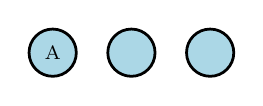
\begin{tikzpicture}
    \Vertex[IdAsLabel]{A}
    \Vertex[x=1,label=B,NoLabel]{B}
    \Vertex[x=2,IdAsLabel,NoLabel]{C}
    \end{tikzpicture}
\end{minipage}

\verb|\Vertex[<Math>,<label>=string]{Name}|

选项 \verb|<Math>| 允许将标签转换为数学
不使用\$ \$环境的表达式。 结合
与 \verb|<IdAsLabel>| 允许这个选项也数学表达式
通过顶点名称的定义。

\begin{minipage}[c]{0.55\textwidth}
  \centering
  \begin{lstlisting}[gobble=8]
        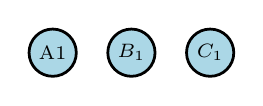
\begin{tikzpicture}
         \Vertex[IdAsLabel]{A1} % 分配顶点标签
         \Vertex[x=1,label=B _ 1,Math]{B} % 运用数学标签,但是不需要添加数学环境
         \Vertex[x=2,Math,IdAsLabel]{C _ 1} % 运用数学环境不需要添加数学环境
        \end{tikzpicture}
  \end{lstlisting}
\end{minipage}
\hfil
\begin{minipage}[c]{0.40\textwidth}
  \centering
  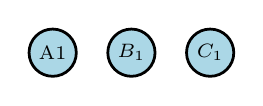
\begin{tikzpicture}
    \Vertex[IdAsLabel]{A1}
    \Vertex[x=1,label=B _ 1,Math]{B}
    \Vertex[x=2,Math,IdAsLabel]{C _ 1}
    \end{tikzpicture}
\end{minipage}



\verb|\Vertex[<RGB>,<color>=RGB values]{Name}|

为了显示RGB顶点填充颜色,可选项
必须输入 \verb|<RGB>|。 结合此选项,
\verb|<color>|我不必是带有 RGB 值的列表,并用","和
内 \{ \}

\begin{minipage}[c]{0.55\textwidth}
  \centering
  \begin{lstlisting}[gobble=8]
    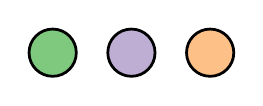
\begin{tikzpicture}
      \Vertex[RGB,color={127,201,127}]{A} % 进行了颜色填充,默认位置为原点
      \Vertex[x=1,RGB,color={190,174,212}]{B} % 进行位置设定和颜色填充
      \Vertex[x=2,RGB,color={253,192,134}]{C} % 进行颜色色设定和位置
      \end{tikzpicture}
  \end{lstlisting}
\end{minipage}
\hfil
\begin{minipage}[c]{0.40\textwidth}
  \centering
     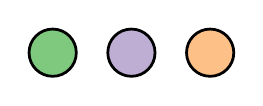
\begin{tikzpicture}
      \Vertex[RGB,color={127,201,127}]{A}
      \Vertex[x=1,RGB,color={190,174,212}]{B}
      \Vertex[x=2,RGB,color={253,192,134}]{C}
     \end{tikzpicture}
\end{minipage}




\verb|\Vertex[<Pseudo>]{Name}|

选项 \verb|<Pseudo>| 创建一个伪顶点,其中仅
将绘制顶点名称和顶点坐标。 边缘等
仍可以分配给该顶点。

\begin{minipage}[c]{0.55\textwidth}
  \centering
  \begin{lstlisting}[gobble=8]
        
\begin{tikzpicture}
          \Vertex{A}
           \Vertex[x=2,Pseudo]{B} %
         \end{tikzpicture}
  \end{lstlisting}
\end{minipage}
\hfil
\begin{minipage}[c]{0.40\textwidth}
  \centering
  
\begin{tikzpicture}
    \Vertex{A}
    \Vertex[x=2,Pseudo]{B}
    \end{tikzpicture}
\end{minipage}


\verb|\Vertex[<layer>]{Name}|

使用选项 \verb|<layer>|,可以将顶点分配给特定的
层。 有关此选项的更多信息,以及层的使用,请参见
第 4 章。

\subsection{顶点连边的绘制/输入(Edge)}

第二个基本命令是\verb|\Edge|,用于连接两个顶点。

可以在一个或两个顶点之间生成边。 在第一
在这种情况下,将生成一个自循环。 作为强制性论据
必须输入应该连接的顶点的名称
在()中。 在有向边的情况下,顺序很重要的点是; 从 Vertexi(原点)到 Vertexj(destination)。

对于 \verb|\Edge|,可以使用以下选项:

%tab2
\begin{table}[h!t]
  \center
  \renewcommand\arraystretch{0.8}
  \tabcolsep 10pt
    \caption{Local Options for the Edge
    Command}
  \begin{tabular}{p{60pt}<{\raggedright}p{40pt}<{\raggedright}p{50pt}<{\raggedright}p{150pt}<{\raggedright}}
\hline\\[-4.5mm]\hline
Option &    Default  &   Type  &   Definition\\
\hline
lw &  \{\}  & measure &  line width of the edge\\
color &  \{\}  & color e & dge color\\
opacity &  \{\} &  number &  opacity of the edge\\
bend &  0  & number &  angle out/in of the vertex\\
label  & \{\}  & string &  label\\
fontsize &\{\}  & string &  font size of the label\\
fontcolor &  \{\}  & color &  font color of the label\\
fontscale &  \{\}  & number &  scale of the label\\
position  & \{\}  & string &  label position\\
distance &  0.5  & number &  label distance from vertex i\\
style &  \{\}  & string  & additional\textcolor{black}{Ti\textcolor{orange}{\emph{k}}Z} styles\\
path &  \{\} &  list  & path over several vertices\\
loopsize &  1cm &  measure &  size parameter of the self-loop\\
loopposition &  0 &  number &  orientation of the self-loop\\
loopshape &  90  & number  & loop angle out/in of the vertex\\
Direct  & false &  Boolean &  allow directed edges\\
Math  & false  & Boolean &  displays the label in math mode\\
RGB &  false &  Boolean &  allow RGB colors\\
NotInBG &  false &  Boolean  & edge is not in the background layer\\
\hline\\[-4.5mm]\hline
%\multicolumn{4}{c}{either measure or string}
  \end{tabular}
\end{table}

可选参数;\verb|<loopsize>|、\verb|<loopposition>|,\verb|<loopsize>|仅用于自循环可选参数。

\verb|\Edge(Vertexi)(Vertexj)|

在两个顶点之间连接一条边;

\begin{minipage}[c]{0.55\textwidth}
  \centering
  \begin{lstlisting}[gobble=8]
        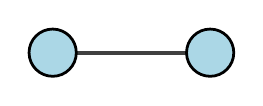
\begin{tikzpicture}
          \Vertex{A} \Vertex[x=2]{B} % 定位两个顶点
          \Edge(A)(B) % 在两个顶点之间连接一条边
        \end{tikzpicture}
  \end{lstlisting}
\end{minipage}
\hfil
\begin{minipage}[c]{0.40\textwidth}
  \centering
  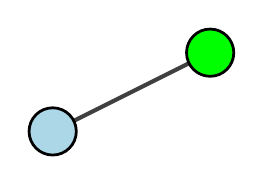
\begin{tikzpicture}
    \Vertex{A} \Vertex[x=2,y=1,color=green]{B}
    \Edge(A)(B)
    \end{tikzpicture}
\end{minipage}

\verb|\Edge[<lw>=measure](Vertexi)(Vertexj)|

连接两个顶点时间的线条粗细可以通过上面的命令进行控制;

\begin{minipage}[c]{0.55\textwidth}
  \centering
  \begin{lstlisting}[gobble=8]
        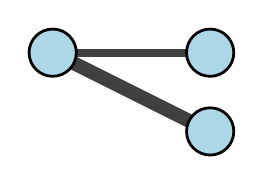
\begin{tikzpicture}
         \Vertex{A} \Vertex[x=2]{B} \Vertex[x=2,y=-1]{C}
         \Edge[lw=3pt](A)(B)
         \Edge[lw=5pt](A)(C)
        \end{tikzpicture}
  \end{lstlisting}
\end{minipage}
\hfil
\begin{minipage}[c]{0.40\textwidth}
  \centering
  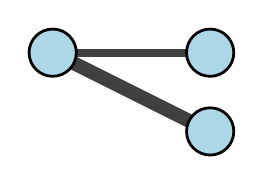
\begin{tikzpicture}
    \Vertex{A} \Vertex[x=2]{B} \Vertex[x=2,y=-1]{C}
    \Edge[lw=3pt](A)(B)
    \Edge[lw=5pt](A)(C)
    \end{tikzpicture}
\end{minipage}

\verb|\Edge[<color>=color](Vertexi)(Vertexj)|

连接两个顶点线条命令的颜色设置;

\begin{minipage}[c]{0.55\textwidth}
  \centering
  \begin{lstlisting}[gobble=8]
        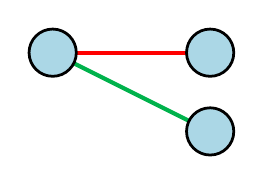
\begin{tikzpicture}
         \Vertex{A} \Vertex[x=2]{B} \Vertex[x=2,y=-1]{C}
         \Edge[color=red](A)(B)
         \Edge[color=green!70!blue](A)(C)
        \end{tikzpicture}
  \end{lstlisting}
\end{minipage}
\hfil
\begin{minipage}[c]{0.40\textwidth}
  \centering
  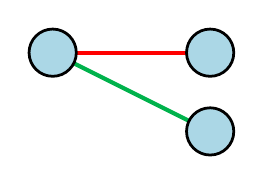
\begin{tikzpicture}
    \Vertex{A} \Vertex[x=2]{B} \Vertex[x=2,y=-1]{C}
    \Edge[color=red](A)(B)
    \Edge[color=green!70!blue](A)(C)
    \end{tikzpicture}
\end{minipage}

\verb|\Edge[<opacity>=number](Vertexi)(Vertexj)|

用上述命令进行对连接顶点的边的透明度进行设定,设置的值在 [0,1] 之间;

\begin{minipage}[c]{0.55\textwidth}
  \centering
  \begin{lstlisting}[gobble=8]
         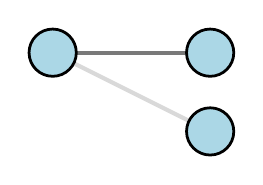
\begin{tikzpicture}
         \Vertex{A} \Vertex[x=2]{B} \Vertex[x=2,y=-1]{C}
         \Edge[opacity=.7](A)(B)
         \Edge[opacity=.2](A)(C)
        \end{tikzpicture}
  \end{lstlisting}
\end{minipage}
\hfil
\begin{minipage}[c]{0.40\textwidth}
  \centering
     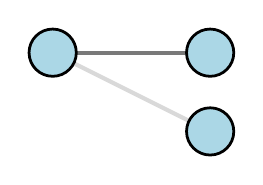
\begin{tikzpicture}
       \Vertex{A} \Vertex[x=2]{B} \Vertex[x=2,y=-1]{C}
       \Edge[opacity=.7](A)(B)
       \Edge[opacity=.2](A)(C)
     \end{tikzpicture}
\end{minipage}

连接顶点的边的透明度可选参数可以对边进行改变;另外,在连接顶点之间的线条时,我们还可以通过曲线去连接,通过命令:

\verb|\Edge<bend>=number](Vertex i)(Vertexj)|

可以使用~\verb|<bend>|选项修改边缘的形状。 如果
在顶点之间绘制直线时,未指定任何内容。
该数字定义边缘偏离的角度
它的直接联系。 正数会使边缘计数器弯曲
顺时针旋转,而负数使顺时针旋转。

\begin{minipage}[c]{0.55\textwidth}
  \centering
  \begin{lstlisting}[gobble=8]
         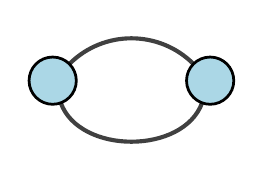
\begin{tikzpicture}
           \Vertex{A} \Vertex[x=2]{B}
           \Edge[bend=45](A)(B)
          \Edge[bend=-70](A)(B)
         \end{tikzpicture}
  \end{lstlisting}
\end{minipage}
\hfil
\begin{minipage}[c]{0.40\textwidth}
  \centering
  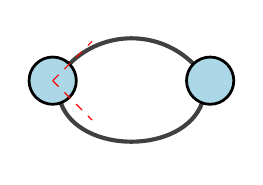
\begin{tikzpicture}
    \Vertex{A} \Vertex[x=2]{B}
    \Edge[bend=45](A)(B)
    \Edge[bend=-70](A)(B)
    \draw[red,dashed](0,0)--(.5,.5)(0,0)--(.5,-.5);
    \end{tikzpicture}
\end{minipage}

\verb|\Edge<label>=string](Vertexi)(Vertexj)|

在连接定点的边时,我们还可以设置连接顶点变的命名;

边缘用选项 \verb|<label>| 标记。 对于任何标签
可以使用字符串参数,包括空格。 数学环境 \$ \$ 可用于显示数学表达式。

\begin{minipage}[c]{0.55\textwidth}
  \centering
  \begin{lstlisting}[gobble=8]
        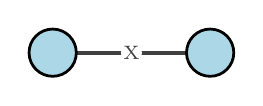
\begin{tikzpicture}
         \Vertex{A} \Vertex[x=2]{B}
         \Edge[label=X](A)(B)
        \end{tikzpicture}
  \end{lstlisting}
\end{minipage}
\hfil
\begin{minipage}[c]{0.40\textwidth}
  \centering
  \begin{tikzpicture}
    \Vertex{A} \Vertex[x=2]{B}
    \Edge[label=X](A)(B)
  \end{tikzpicture}
\end{minipage}

\verb|\Edge<label>=string,<fontsize>=string](Vertexi)(Vertexj)|

标签字体的大小可以通过命令:

\verb|<\fontsize>=string(\tiny/\scriptsize/\footnotesize/\small/\large/\Large...|
进行修改,

\verb|<label>| 的字体大小可以通过以下选项进行修改
\verb|<fontsize>|。 这里可以使用常用的 \LaTeX{} 字体大小命令
\verb|\tiny/\scriptsize/\footnotesize/\small/....|
更改标签的大小。

\begin{minipage}[c]{0.55\textwidth}
  \centering
  \begin{lstlisting}[gobble=8]
        \begin{tikzpicture}
          \Vertex{A} \Vertex[x=2]{B} \Vertex[x=2,y=-1]{C}
          \Edge[label=X,fontsize=\large](A)(B)
          \Edge[label=Y,fontsize=\tiny](A)(C)
        \end{tikzpicture}
  \end{lstlisting}
\end{minipage}
\hfil
\begin{minipage}[c]{0.40\textwidth}
  \centering
  \begin{tikzpicture}
    \Vertex{A} \Vertex[x=2]{B} \Vertex[x=2,y=-1]{C}
    \Edge[label=X,fontsize=\large](A)(B)
    \Edge[label=Y,fontsize=\tiny](A)(C)
    \end{tikzpicture}
\end{minipage}

另外,我们还可以通过命令:

\verb|\Edge[<\label>=string,<fontcolor>=color](Vertexi)(Vertexj)|、来改变变标签的颜色;

\begin{minipage}[c]{0.55\textwidth}
  \centering
  \begin{lstlisting}[gobble=8]
        \begin{tikzpicture}
          \Vertex{A} \Vertex[x=2]{B} \Vertex[x=2,y=-1]{C}
          \Edge[label=X,fontcolor=blue](A)(B)
          \Edge[label=Y,fontcolor=red](A)(C)
         \end{tikzpicture}
  \end{lstlisting}
\end{minipage}
\hfil
\begin{minipage}[c]{0.40\textwidth}
  \centering
  \begin{tikzpicture}
    \Vertex{A} \Vertex[x=2]{B} \Vertex[x=2,y=-1]{C}
    \Edge[label=X,fontcolor=blue](A)(B)
    \Edge[label=Y,fontcolor=red](A)(C)
    \end{tikzpicture}
\end{minipage}

\verb|\Edge[<\label>=string,<fontscale>=number](Vertexi)(Vertexj)|

通过 \verb|<fontscale>| 来控制进行对字体的缩放,它与 \verb|<fontsize>|的功能刚好相反,它本身不会改变字体的大小,只会将当前的字体进行放大或者缩小。

\begin{minipage}[c]{0.55\textwidth}
  \centering
  \begin{lstlisting}[gobble=8]
         \begin{tikzpicture}
          \Vertex{A} \Vertex[x=2]{B} \Vertex[x=2,y=-1]{C}
          \Edge[label=X,fontscale=.5](A)(B)
          \Edge[label=Y,fontscale=2](A)(C)
         \end{tikzpicture}
  \end{lstlisting}
\end{minipage}
\hfil
\begin{minipage}[c]{0.40\textwidth}
  \centering
  \begin{tikzpicture}
    \Vertex{A} \Vertex[x=2]{B} \Vertex[x=2,y=-1]{C}
    \Edge[label=X,fontscale=.5](A)(B)
    \Edge[label=Y,fontscale=2](A)(C)
  \end{tikzpicture}
\end{minipage}

下面,我们对变标签位置可选参数命令进行设定;

\verb|\Edge[<\label>=string,<position>=string](Vertexi)(Vertexj)|

默认条件下标签的位置位于谅解两个点之间的中间,我们可以通过标签位置可选参数进行修改:

\begin{minipage}[c]{0.55\textwidth}
  \centering
  \begin{lstlisting}[gobble=8]
        \begin{tikzpicture}
         \Vertex{A} \Vertex[x=2]{B} \Vertex[x=2,y=-1]{C}
         \Edge[label=X,position=above](A)(B)
         \Edge[label=Y,position={below left=2mm}](A)(C)
        \end{tikzpicture}
  \end{lstlisting}
\end{minipage}
\hfil
\begin{minipage}[c]{0.40\textwidth}
  \centering
  \begin{tikzpicture}
    \Vertex{A} \Vertex[x=2]{B} \Vertex[x=2,y=-1]{C}
    \Edge[label=X,position=above](A)(B)
    \Edge[label=Y,position={below left=2mm}](A)(C)
    \end{tikzpicture}
\end{minipage}

\verb|<distance>|可以用来设定两个顶点之间连边的长度的标签位置,命令为;

\verb|\Edge[<\label>=string,<distance>=number](Vertexi)(Vertexj)|

在默认条件下,链接两个顶点的边在具体的输入number数字后,表示将连边的长度进行乘上倍数,就是标签所在为相应方向上的相对位置。

\begin{minipage}[c]{0.55\textwidth}
  \centering
  \begin{lstlisting}[gobble=8]
         \begin{tikzpicture}
         \Vertex{A} \Vertex[x=2]{B}
         \Edge[label=X,distance=.7](A)(B)
         \end{tikzpicture}\quad
         \begin{tikzpicture}
          \Vertex{A} \Vertex[x=3]{B}
          \Edge[label=X,distance=0.3](A)(B)
          \end{tikzpicture}
  \end{lstlisting}
\end{minipage}
\hfil
\begin{minipage}[c]{0.40\textwidth}
  \centering
  \begin{tikzpicture}
    \Vertex{A} \Vertex[x=2]{B}
    \Edge[label=X,distance=.7](A)(B)
    \end{tikzpicture}\\
    \begin{tikzpicture}
     \Vertex{A} \Vertex[x=3]{B}
     \Edge[label=X,distance=0.3](A)(B)
     \end{tikzpicture}
\end{minipage}

\verb|\Edge[<style>=string](Vertexi)(Vertexj)|

运用虚线连接边;

\begin{minipage}[c]{0.55\textwidth}
  \centering
\begin{lstlisting}[gobble=8]
        \begin{tikzpicture}
         \Vertex{A} \Vertex[x=2]{B}
         \Edge[style={dashed}](A)(B)
        \end{tikzpicture}
  \end{lstlisting}
\end{minipage}
\hfil
\begin{minipage}[c]{0.40\textwidth}
  \centering
  \begin{tikzpicture}
    \Vertex{A} \Vertex[x=2]{B}
    \Edge[style={dashed}](A)(B)
    \end{tikzpicture}
\end{minipage}

连接边的路径设置,用用命令;\verb|\Edge[<path>=list](Vertexi)(Vertexj)|

\begin{minipage}[c]{0.55\textwidth}
  \centering
  \begin{lstlisting}[gobble=8]
        \begin{tikzpicture}
        \Vertex{A} \Vertex[x=2]{B} \Vertex[x=2,y=-1]{C}
        \Edge[path={A,{0,-1},C,B}](A)(B)
        \end{tikzpicture}
  \end{lstlisting}
\end{minipage}
\hfil
\begin{minipage}[c]{0.40\textwidth}
  \centering
  \begin{tikzpicture}
    \Vertex{A} \Vertex[x=2]{B} \Vertex[x=2,y=-1]{C}
    \Edge[path={A,{0,-1},C,B}](A)(B)
    \end{tikzpicture}
\end{minipage}

为了绘制连接一系列顶点和/或坐标的边的有限序列,选项\verb|<path>|可以是用过。 此选项的参数必须是列表元素. 当前标签和弯曲
不支持边缘!由\{\}括号组成,包含中间名称
顶点。 新坐标(即没有顶点)可以位于
与\verb|{h<x>=numbber,<y>=number}|。 列表的参数必须由分隔
逗号“,”。

\verb|\Edge(Vertexi)(Vertexj)|

通过使用与原点相同的顶点和
目的地。 除了上述选项外,还有三个
自循环特定的选项:

\verb|<loopsize>|,\verb|<loopposition>|和 \verb|<loopshape>|。

\begin{minipage}[c]{0.55\textwidth}
  \centering
  \begin{lstlisting}[gobble=8]
        \begin{tikzpicture}
         \Vertex{A}
         \Edge(A)(A)
        \end{tikzpicture}
  \end{lstlisting}
\end{minipage}
\hfil
\begin{minipage}[c]{0.40\textwidth}
  \centering
  \begin{tikzpicture}
    \Vertex{A}
    \Edge(A)(A)
    \end{tikzpicture}
\end{minipage}

进一步我们可以设定自循环边的大小,通过命令;

\verb|\Edge[<loopsize>=maesure](Vertexi)(Vertexi)|

默认条件下,默认值为 1~cm,

\begin{minipage}[c]{0.55\textwidth}
  \centering
  \begin{lstlisting}[gobble=8]
        \begin{tikzpicture}
        \Vertex{A} \Vertex[x=1.3]{B}
        \Edge[loopsize=.5cm](A)(A)
        \Edge[loopsize=1.5cm](B)(B)
        \end{tikzpicture}
  \end{lstlisting}
\end{minipage}
\hfil
\begin{minipage}[c]{0.40\textwidth}
  \centering
  \begin{tikzpicture}
    \Vertex{A} \Vertex[x=1.3]{B}
    \Edge[loopsize=.5cm](A)(A) % 方向默认为在右边
    \Edge[loopsize=1.5cm](B)(B)
    \end{tikzpicture}
\end{minipage}

我们可以在自循环中设置路径的位置,主要是通过命令 \verb|\Edge[<loopposition>=number]|

\verb|(Vertexi)(Vertexi)| 旋转角度来进行改变;

\verb|\Edge[<loopsize>=maesure](Vertexi)(Vertexi)|

\begin{minipage}[c]{0.55\textwidth}
  \centering
  \begin{lstlisting}[gobble=8]
          \begin{tikzpicture}
           \Vertex{A} \Vertex[x=1.5]{B}
           \Edge[loopposition=45](A)(A)
           \Edge[loopposition=-70](B)(B)
          \end{tikzpicture}
  \end{lstlisting}
\end{minipage}
\hfil
\begin{minipage}[c]{0.40\textwidth}
  \centering
  \begin{tikzpicture}
    \Vertex{A} \Vertex[x=1.5]{B}
    \Edge[loopposition=45](A)(A)
    \Edge[loopposition=-70](B)(B)
    \end{tikzpicture}
\end{minipage}

自循环由包围角度角度来确定,我们可以通过可选参数命令 \verb|<loopshape>|来进行改变这个角度。

\verb|\Edge[<loopshape>=maesure](Vertexi)(Vertexi)|

\begin{minipage}[c]{0.55\textwidth}
  \centering
  \begin{lstlisting}[gobble=8]
        \begin{tikzpicture}
        \Vertex{A}
        \Edge[loopshape=45](A)(A)
        \end{tikzpicture}
  \end{lstlisting}
\end{minipage}
\hfil
\begin{minipage}[c]{0.40\textwidth}
  \centering
  \begin{tikzpicture}
    \Vertex{A}
    \Edge[loopshape=45](A)(A)
    \end{tikzpicture}
\end{minipage}

我们可以通过如下命令进行改变连接顶点边指向箭头;

\verb|\Edge[<Direct>](Vertexi)(Vertexj)|

\begin{minipage}[c]{0.55\textwidth}
  \centering
  \begin{lstlisting}[gobble=8]
      \begin{tikzpicture}
      \Vertex{A} \Vertex[x=2]{B}
      \Edge[Direct](A)(B)
      \end{tikzpicture}
  \end{lstlisting}
\end{minipage}
\hfil
\begin{minipage}[c]{0.40\textwidth}
  \centering
     \begin{tikzpicture}
      \Vertex{A} \Vertex[x=2]{B}
       \Edge[Direct](A)(B)
      \end{tikzpicture}
\end{minipage}

连接顶点的连接边的数学标签,通过~\verb|<Math>| 进行可选参数的值进行修改;

\verb|\Edge[Math,label=<string>](Vertexi)(Vertexj)|

  \begin{minipage}[c]{0.55\textwidth}
    \centering
    \begin{lstlisting}[gobble=8]
        \begin{tikzpicture}
        \Vertex{A} \Vertex[x=2]{B}
        \Edge[Math,label=X _ 1](A)(B)
        \end{tikzpicture}
    \end{lstlisting}
  \end{minipage}
  \hfil
  \begin{minipage}[c]{0.40\textwidth}
    \centering
    \begin{tikzpicture}
      \Vertex{A} \Vertex[x=2]{B}
      \Edge[Math,label=X _ 1](A)(B)
      \end{tikzpicture}
  \end{minipage}

  对于连接边的颜色设定;通过可选参数~\verb|<RGB value>| 来进行改变,

  \verb|\Edge[RGB,color=<RGB value>](Vertexi)(Vertexj)|

  \begin{minipage}[c]{0.55\textwidth}
    \centering
    \begin{lstlisting}[gobble=8]
        \begin{tikzpicture}
        \Vertex{A} \Vertex[x=2]{B} \Vertex[x=2,y=-1]{C}
        \Edge[RGB,color={127,201,127}](A)(B)
        \Edge[RGB,color={253,192,134}](A)(C)
        \end{tikzpicture}
    \end{lstlisting}
  \end{minipage}
  \hfil
  \begin{minipage}[c]{0.40\textwidth}
    \centering
    \begin{tikzpicture}
      \Vertex{A} \Vertex[x=2]{B} \Vertex[x=2,y=-1]{C}
      \Edge[RGB,color={127,201,127}](A)(B)
      \Edge[RGB,color={253,192,134}](A)(C)
      \end{tikzpicture}
  \end{minipage}

  \verb|\Edge[<RGB value>](Vertexi)(Vertexj)|

  默认情况下,边缘绘制在
  \textcolor{black}{Ti\textcolor{orange}{\emph{k}}Z}-\textcolor{blue}{picture}。 即 边缘出现后创建的对象
  在他们之上。 要关闭此功能,我拥有的选项 <NotInBG>
  启用。 可以使用以下方法更改默认设置
  \verb|\EdgesNotInBG|或\verb|\EdgesInBG|

  \begin{minipage}[c]{0.55\textwidth}
    \centering
    \begin{lstlisting}[gobble=8]
        \begin{tikzpicture}
        \Vertex{A} \Vertex[x=2]{B} \Vertex[x=1,y=-.5]{C}
        \Vertex[y=-1]{D} \Vertex[x=2,y=-1]{E}
        \Edge[bend=-30](A)(B)
        \Edge[bend=30,NotInBG](D)(E)
        \end{tikzpicture}
    \end{lstlisting}
  \end{minipage}
  \hfil
  \begin{minipage}[c]{0.40\textwidth}
    \centering
    \begin{tikzpicture}
      \Vertex{A} \Vertex[x=2]{B} \Vertex[x=1,y=-.5]{C}
      \Vertex[y=-1]{D} \Vertex[x=2,y=-1]{E}
      \Edge[bend=-30](A)(B)
      \Edge[bend=30,NotInBG](D)(E)
      \end{tikzpicture}
  \end{minipage}

\subsection{顶点内容为文本绘制(Text)}

在神经网络图形绘制过程中,有时候顶点可以用文字内容进行在相应的位置进行表示,我们最主要的最简洁的命令就是\verb|\Text|,通过这个命令来完成这个事情。现在相当于将前面的顶点元素当成文字来进行即可。

进行\verb|\Text|命令来进行绘制时的相关的参数设置;


%t3
\begin{table}[h!]
  \center
  \tabcolsep 6pt
  \renewcommand\arraystretch{0.8}
    \caption{Local Options for The Text
    Command}
  \begin{tabular}{p{60pt}<{\raggedright}p{40pt}<{\raggedright}p{50pt}<{\raggedright}p{150pt}<{\raggedright}}
\hline\\[-4.5mm]\hline
Option &    Default  &   Type  &   Definition\\
\hline
x &  0  & measure &   x-coordinate\\
y &  0 &  measure &  y-coordinate\\
fontsize &  \{\}  & fontsize &  font size of the text\\
color &  \{\} &  color &  color of the text\\
opacity &\{\} &  number &  opacity of the text\\
position &  center &  string &  position of the text to the origin\\
distance &  0cm &  measure &  distance from the origin\\
rotation &  0 &  number &  rotation of the text\\
anchor &  \{\} &  string &  anchor of the text\\
width &  \{\}  & number &  width of the text box\\
style &  \{\} &  string &  additional\textcolor{black}{Ti\textcolor{orange}{\emph{k}}Z} styles\\
layer &  \{\} &  number &  assigned layer of the text\\
RGB &  false  & Boolean &  allow RGB colors\\
\hline\\[-4.5mm]\hline
  \end{tabular}

\end{table}

为准确无误的将一些可选参数对默认的值进行修改,我们可以通过命令\verb|\SetTextStyle| 来实现,

\verb|\Text[<x>=measure,<y>=measure]{string}|

在没有赋予横纵坐标相应的值是,一般默认为原点;

\begin{minipage}[c]{0.55\textwidth}
  \centering
  \begin{lstlisting}[gobble=8]
        \begin{tikzpicture}
         \Text{A} % 默认在原点位置
         \Text[x=1,y=1]{B} % 在坐标(1,1)位置
         \Text[x=2]{C} % 在坐标(2,0)位置
        \end{tikzpicture}
  \end{lstlisting}
\end{minipage}
\hfil
\begin{minipage}[c]{0.40\textwidth}
  \centering
  \begin{tikzpicture}
    \Text{A}
    \Text[x=1,y=1]{B}
    \Text[x=2]{C}
    \end{tikzpicture}
\end{minipage}

对文本字体的大小设置:

\verb|\Text[<fontsize>=fontsize(\tiny/\scriptsize/small/|

\verb|\footnotesize\normalsize\large...)]{string}|

\begin{minipage}[c]{0.55\textwidth}
  \centering
  \begin{lstlisting}[gobble=8]
        \begin{tikzpicture}
        \Text[fontsize=\small]{A}
        \Text[x=1,fontsize=\LARGE]{B}
        \Text[x=2,fontsize=\Huge]{C}
        \end{tikzpicture}
  \end{lstlisting}
\end{minipage}
\hfil
\begin{minipage}[c]{0.40\textwidth}
  \centering
  \begin{tikzpicture}
    \Text[fontsize=\small]{A}
    \Text[x=1,fontsize=\LARGE]{B}
    \Text[x=2,fontsize=\Huge]{C}
    \end{tikzpicture}
\end{minipage}

对文本文字内容颜色的设置;

\verb|\Text[<color>=colo]{string}|

\begin{minipage}[c]{0.55\textwidth}
  \centering
  \begin{lstlisting}[gobble=8]
         \begin{tikzpicture}
          \Text[color = blue]{A}
          \Text[x=1,color=red]{B}
          \Text[x=2,color=green!70!blue]{C}
         \end{tikzpicture}
  \end{lstlisting}
\end{minipage}
\hfil
\begin{minipage}[c]{0.40\textwidth}
  \centering
  \begin{tikzpicture}
    \Text[color = blue]{A}
    \Text[x=1,color=red]{B}
    \Text[x=2,color=green!70!blue]{C}
    \end{tikzpicture}
\end{minipage}

透明度设置;

\verb|<opacity>=number]{string}|

\begin{minipage}[c]{0.55\textwidth}
  \centering
  \begin{lstlisting}[gobble=8]
        \begin{tikzpicture}
         \Text[opacity = 1]{A}
         \Text[x=1,opacity =.7]{B}
         \Text[x=2,opacity =.2]{C}
        \end{tikzpicture}
  \end{lstlisting}
\end{minipage}
\hfil
\begin{minipage}[c]{0.40\textwidth}
  \centering
  \begin{tikzpicture}
    \Text[opacity = 1]{A}
    \Text[x=1,opacity =.7]{B}
    \Text[x=2,opacity =.2]{C}
    \end{tikzpicture}
\end{minipage}

位置和间距设置

\verb|<position>=number,<distance>=measure>]{string}|

\begin{minipage}[c]{0.55\textwidth}
  \centering
  \begin{lstlisting}[gobble=8]
        \begin{tikzpicture}
         \Text[position=above]{above}
         \Text[position=below]{below}
         \Text[position=left,distance=5mm]{left}
         \Text[position=above right,distance=5mm]{above right}
        \end{tikzpicture}
  \end{lstlisting}
\end{minipage}
\hfil
\begin{minipage}[c]{0.40\textwidth}
  \centering
    \begin{tikzpicture}
      \Text[position=above]{above}
      \Text[position=below]{below}
      \Text[position=left,distance=5mm]{left}
      \Text[position=above right,distance=5mm]{above right}
      \end{tikzpicture}
\end{minipage}

文字内容设置旋转;

\verb|<rotation>=number]{string}|

\begin{minipage}[c]{0.55\textwidth}
  \centering
  \begin{lstlisting}[gobble=8]
         \begin{tikzpicture}
          \Text[rotation=30]{A}
          \Text[x=1,rotation=45]{B}
          \Text[x=2,rotation=75]{C}
         \end{tikzpicture}
  \end{lstlisting}
\end{minipage}
\hfil
\begin{minipage}[c]{0.40\textwidth}
  \centering
  \begin{tikzpicture}
    \Text[rotation=30]{A}
    \Text[x=1,rotation=45]{B}
    \Text[x=2,rotation=75]{C}
    \end{tikzpicture}
\end{minipage}

\verb|\Text[<anchor>=string]{string}|

用来设置内容在指定位置的那一个方位

\begin{minipage}[c]{0.55\textwidth}
  \centering
  \begin{lstlisting}[gobble=8]
         \begin{tikzpicture}
          \Text[anchor=north east]{NE}
          \Text[x=1,anchor = south]{S}
          \Text[x=2,anchor =south west]{SW}
         \end{tikzpicture}
  \end{lstlisting}
\end{minipage}
\hfil
\begin{minipage}[c]{0.40\textwidth}
  \centering
  \begin{tikzpicture}
    \Text[anchor=north east]{NE}
    \Text[x=1,anchor = south]{S}
    \Text[x=2,anchor =south west]{SW}
    \end{tikzpicture}
\end{minipage}

位置文本内容的长度进行设置

\verb|\Text[<width>=number]{string}|

\begin{minipage}[c]{0.55\textwidth}
  \centering
  \begin{lstlisting}[gobble=8]
         \begin{tikzpicture}
         \Text[width=2.5cm]{This might be a very long text.}
         \end{tikzpicture}
  \end{lstlisting}
\end{minipage}
\hfil
\begin{minipage}[c]{0.40\textwidth}
  \centering
  \begin{tikzpicture}
    \Text[width=2.5cm]{This might be a very long text.}
    \end{tikzpicture}
\end{minipage}

另外相关的风格设置命令~\verb|<style>|进行\textcolor{black}{Ti\textcolor{orange}{\emph{k}}Z}/PGF相关风格的设置。

\begin{minipage}[c]{0.55\textwidth}
  \centering
  \begin{lstlisting}[gobble=8]
         \begin{tikzpicture}
          \Text[style={draw,rectangle}]{A}
          \Text[x=1,style={fill=red}]{B}
          \Text[x=2,style={fill=blue,circle,opacity=.3}]{C}
         \end{tikzpicture}
  \end{lstlisting}
\end{minipage}
\hfil
\begin{minipage}[c]{0.40\textwidth}
  \centering
  \begin{tikzpicture}
    \Text[style={draw,rectangle}]{A}
    \Text[x=1,style={fill=red}]{B}
    \Text[x=2,style={fill=blue,circle,opacity=.3}]{C}
    \end{tikzpicture}
\end{minipage}

运用命令~\verb|<RGB>| 对内容颜色、填充,阴影等进行设置

\verb|\Text[RGB,<color>=RGB values]{string}|

\begin{minipage}[c]{0.55\textwidth}
  \centering
  \begin{lstlisting}[gobble=8]
         \begin{tikzpicture}
          \Text[RGB,color={127,201,127}]{A}
          \Text[x=1,RGB,color={190,174,212}]{B}
          \Text[x=2,RGB,color={253,192,134}]{C}
         \end{tikzpicture}
  \end{lstlisting}
\end{minipage}
\hfil
\begin{minipage}[c]{0.40\textwidth}
  \centering
  \begin{tikzpicture}
    \Text[RGB,color={127,201,127}]{A}
    \Text[x=1,RGB,color={190,174,212}]{B}
    \Text[x=2,RGB,color={253,192,134}]{C}
    \end{tikzpicture}
\end{minipage}

%3
\section{复杂(多元)神经网络图形绘制/输入(Complex Networks)}

虽然在第2章中介绍了网络的构建块,但是~\textcolor{black}{Ti\textcolor{orange}{\emph{k}}Z}-\textcolor{blue}{network} 软件包的主要优点是可以更好地进行解释。 这包括根据获得的数据创建网络
来自其他来源(例如 Python,R,GIS)。 想法是布局将由此外部源完成,并使用\textcolor{black}{Ti\textcolor{orange}{\emph{k}}Z}-\textcolor{blue}{network}进行一些更改,然后在\LaTeX{}中重新创建网络。

% 3.1
\subsection{顶点集合的绘制(Vertices)}

\verb|Vertices|命令是\verb|\Vertex|命令的扩展。将会绘制一组顶点,而不是单个顶点。这套的顶点数在外部文件中定义,但可以使用\verb|\Vertices|。\verb|\Vertices| \verb|[<global options>] {filename}|

\verb|[<global options>] {filename}|

顶点必须存储在明文文件1中,优先例如.txt,.tex,.csv,.dat ...以.csv格式。第一行应包含标题,等于表~2.1 中定义的选项。选项分开用逗号“,”。每个新行都对应一个新顶点。

\begin{lstlisting}
  id, x, y ,size,color ,opacity,label,IdAsLabel,NoLabel % 名称
  A, 0, 0, .4 ,green , .9 , a , false , false % A 点设置相关
  B, 1, .7, .6 , , .5 , b , false , false
  C, 2, 1, .8 ,orange, .3 , c , false , true
  D, 2, 0, .5 ,red , .7 , d , true , false
  E,.2,1.5, .5 ,gray , , e , false , false
\end{lstlisting}

只有~\verb|<id>| 值对于顶点是必需的,并且对应到单个~\verb|\Vertex| 的 <Name> 参数。所以一样
规则和命名约定适用于Name参数:没有数学表达式,没有空格,而且我必须知道
独一无二!所有其他选项都是可选的。没有具体的顺序选项必须保持。如果没有为选项输入任何值,
将选择默认值。文件名不能包含(这不适用于布尔选项,此处为所有值必须输入顶点)。
空格或特殊字符。顶点由命令 \verb|\Vertex|,并加上文件名和文件格式(例如.csv)。如果
顶点文件与主~\LaTeX{} 文件不在同一目录中,还必须指定路径。

\begin{minipage}[c]{0.55\textwidth}
  \centering
  \begin{lstlisting}[gobble=8]
         \begin{tikzpicture}
          \Vertices{vertices.csv}
         \end{tikzpicture}
  \end{lstlisting}
\end{minipage}
\hfil
\begin{minipage}[c]{0.40\textwidth}
  \centering
  \begin{tikzpicture}
    \Vertices{vertices.csv}
    \end{tikzpicture}
\end{minipage}

预定义的 \verb|\Vertex|选项可以被 <global> 操作否决。
\verb|\Vertices|命令的; 即 这些选项适用于所有文件中的顶点。 对于~\verb|\Vertices|,以下选项是
可用的:


%t4
\begin{table}[h!]
  \center
  \tabcolsep 6pt
  \renewcommand\arraystretch{0.75}
    \caption{ Global Options for the
    Vertices Command}
  \begin{tabular}{p{60pt}<{\raggedright}p{40pt}<{\raggedright}p{50pt}<{\raggedright}p{150pt}<{\raggedright}}
\hline\\[-4.3mm]\hline
Option &    Default  &   Type  &   Definition\\
\hline
size &  \{\} &  measure &  diameter of the circles\\
color &  \{\} &  color &  fillcolor of vertices\\
opacity &  \{\} &  number &  opacity of the fill color\\
style &  \{\} &  string &  additional\textcolor{black}{Ti\textcolor{orange}{\emph{k}}Z} styles\\
layer &  \{\} &  number &  assigned layer of the vertices\\
NoLabel &  false &  Boolean &  delete the labels\\
IdAsLabel &  false &  Boolean &  uses the Names as labels\\
Math &  false &  Boolean &  displays the labels in math mode\\
RGB &  false &  Boolean &  allow RGB colors\\
Pseudo &  false &  Boolean &  create a pseudo vertices\\
\hline\\[-4.3mm]\hline
  \end{tabular}

\end{table}

这些可选参数的设定和第~2 章中~\verb|\Vertices|是相似的

下面对文件顶点的大小进行设定更改;顶点的直径可以通过选择来改变我的大小。 默认情况下,顶点的直径为~0.6~厘米。 另外,这里
默认单位为厘米,不必添加到度量中。


\verb|\Vertex[<size>=measure]{filename}|

\begin{minipage}[c]{0.55\textwidth}
  \centering
  \begin{lstlisting}[gobble=8]
         \begin{tikzpicture}
           \Vertices[size=.6]{vertices.csv}
         \end{tikzpicture}
  \end{lstlisting}
\end{minipage}
\hfil
\begin{minipage}[c]{0.40\textwidth}
  \centering
  \begin{tikzpicture}
    \Vertices[size=.6]{vertices.csv}
    \end{tikzpicture}
\end{minipage}

我们还可以对颜色进行对整个文件的顶点进行更改,运用命令;

\verb|\Vertex[<size>=measure]{filename}|

来对文件中所有顶点进行颜色(填充)的更改。

\begin{minipage}[c]{0.55\textwidth}
  \centering
  \begin{lstlisting}[gobble=8]
         \begin{tikzpicture}
          \Vertices[color=green!70!blue]{vertices.csv}
         \end{tikzpicture}
  \end{lstlisting}
\end{minipage}
\hfil
\begin{minipage}[c]{0.40\textwidth}
  \centering
  \begin{tikzpicture}
    \Vertices[color=green!70!blue]{vertices.csv}
    \end{tikzpicture}
\end{minipage}

对于整个文件全局性的顶点的透明度进行更改,我们使用命令:

\verb|\Vertex[<opacity>=number]{filename}|

\begin{minipage}[c]{0.55\textwidth}
  \centering
  \begin{lstlisting}[gobble=8]
         \begin{tikzpicture}
         \Vertices[opacity=.3]{vertices.csv}
         \end{tikzpicture}
  \end{lstlisting}
\end{minipage}
\hfil
\begin{minipage}[c]{0.40\textwidth}
  \centering
  \begin{tikzpicture}
    \Vertices[opacity=.3]{vertices.csv}
    \end{tikzpicture}
\end{minipage}

还可以通过和~\textcolor{black}{Ti\textcolor{orange}{\emph{k}}Z}/PGF 等同的风格设定;具体的命令进行如下:

\verb|[<style>=string]{filename}|

\begin{minipage}[c]{0.55\textwidth}
  \centering
  \begin{lstlisting}[gobble=8]
        \begin{tikzpicture}
         \Vertices[style={shading=ball,blue}]{vertices.csv}
        \end{tikzpicture}
  \end{lstlisting}
\end{minipage}
\hfil
\begin{minipage}[c]{0.40\textwidth}
  \centering
  \begin{tikzpicture}
    \Vertices[style={shading=ball,blue}]{vertices.csv}
    \end{tikzpicture}
\end{minipage}

\verb|[<IdAsLabel>]{filename}|

\verb|[<NoLabel>]{filename}|

\verb|[<IdAsLabel>]|是一个布尔选项,用于分配
单个顶点作为标签。 相反,\verb|[<NoLabel>]|我抑制了所有
标签。

\begin{minipage}[c]{0.55\textwidth}
  \centering
  \begin{lstlisting}[gobble=8]
        \begin{tikzpicture}
         \Vertices[IdAsLabel]{vertices.csv}
        \end{tikzpicture}
  \end{lstlisting}
\end{minipage}
\hfil
\begin{minipage}[c]{0.40\textwidth}
  \centering
  \begin{tikzpicture}
    \Vertices[IdAsLabel]{vertices.csv}
    \end{tikzpicture}
\end{minipage}

\begin{minipage}[c]{0.55\textwidth}
  \centering
  \begin{lstlisting}[gobble=8]
        \begin{tikzpicture}
         \Vertices[NoLabel]{vertices.csv}
        \end{tikzpicture}
  \end{lstlisting}
\end{minipage}
\hfil
\begin{minipage}[c]{0.40\textwidth}
  \centering
  \begin{tikzpicture}
    \Vertices[NoLabel]{vertices.csv}
    \end{tikzpicture}
\end{minipage}

运用颜色~\verb|<RGB>| 对全局的顶点进行设定;

\verb|[<RGB>]{filename}|

为了显示~RGB 顶点填充颜色,可选参数
必须输入 RGB。 此外,RGB 值必须
在存储顶点的文件中指定。 每个值都有
它自己的标题为 <R>,<G> 和 <B>的列

\begin{lstlisting}
  id, x,  y,   size, color, opacity,    label,    R,   G ,    B    % 注意,进行行列对齐,并且严格控制英文逗号
  A,  0,  0,   0.4,  green,     0.9,        a,  255,    0,    0    % 注意可选参数值得取值范围
  B,  1,  0.7, 0.6,       ,     0.5,        b,    0,  255,    0    % 在没有进行参数选择或者是更改时为系统默认
  C,  2,  1,   0.8, orange,     0.3,        c,    0,    0,    255  % 没有进行参数更改时也要注意,用逗号隔开
  D,  2,  0,   0.5,    red,     0.7,        d,   10,  120,    255
  E,  0.2,1.5, 0.5,   gray,        ,        e ,  76,   55,    255
\end{lstlisting}

\begin{minipage}[c]{0.55\textwidth}
  \centering
  \begin{lstlisting}[gobble=8]
         \begin{tikzpicture}
          \Vertices[RGB]{Rvertices.csv}
         \end{tikzpicture}
  \end{lstlisting}
\end{minipage}
\hfil
\begin{minipage}[c]{0.40\textwidth}
  \centering
  \begin{tikzpicture}
    \Vertices[RGB]{Rvertices.csv}
    \end{tikzpicture}
\end{minipage}

\begin{tikzpicture}[multilayer=3d]
  \Plane[x=-.5,y=-.5,width=3,height=2.5]
  \Plane[x=1.7,y=-3.5,width=3,height=2.5,grid=5mm]
  \Vertices{mlvertices.csv}
  \Edges{mledges.csv}
  \end{tikzpicture}

% 3.2
\subsection{边集合网图绘制(Edges)}

命令~\verb|\Edges| 是命令~\verb|\Edge| 命令的扩展使用,适用于多个边连接,相当于集合边的连接,它是一个对全局性的顶点边连接,基础命令为;
\verb|\Edges[<global options>]{filename}|

和顶点全局绘制相类似,在设置边集合文件中,通常为后缀为csv 并且按照给定的表一样进行对应数字补充;每量之间运用英文状态下的逗号“,”隔开,来进行绘制整个边集合的连边。(表格的表头内容是变量 <string>)


\begin{lstlisting}
  u,v,label,lw,color ,opacity,bend, R , G , B ,Direct
  A,B, ab ,.5,red , 1 , 30, 0,120,255,false
  B,C, bc ,.7,blue , 1 , -60, 76, 55,255,false
  B,D, bd ,.5,blue , .5 , -60, 76, 55,255,false
  A,E, ae , 1,green , 1 , 75,255, 0, 0,true
  C,E, ce , 2,orange, 1 , 0,150,150,150,false
  A,A, aa ,.3,black , .5 , 75,255, 0 ,0,false
\end{lstlisting}

强制值是 <u> 和 <v> 参数,其中
对应于单个 \verb|\Edge| 的 <Vertexi> 和 <Vertexj> 参数。
仅当存在具有相同名称的顶点时,才可以创建边。 所有
其他选项是可选的。 选项没有特定的顺序
保持。 如果没有为选项输入任何值,则为默认值
将被选择。 文件名不能包含空格或
待办事项! 这不适用于
布尔选项,此处为所有值
必须输入顶点。
特殊字符。 边缘由命令 \verb|\Edges|绘制
文件名加文件格式(例如.csv)。 如果边缘文件不是
与主 \LaTeX{} 文件位于同一目录中,路径也必须
被指定。 为了绘制边缘,首先必须将顶点
产生。 只有这样,才能分配边。

\begin{minipage}[c]{0.55\textwidth}
  \centering
  \begin{lstlisting}[gobble=8]
         \begin{tikzpicture}
          \Vertices{vertices.csv}
          \Edges{Edges.csv}
         \end{tikzpicture}
  \end{lstlisting}
\end{minipage}
\hfil
\begin{minipage}[c]{0.40\textwidth}
  \centering
  \begin{tikzpicture}
    \Vertices{vertices.csv}
    \Edges{Edges.csv}
    \end{tikzpicture}
\end{minipage}

预定义的~\verb|\Edges| 选项可以被~<global option>
\verb|\Edges| 命令覆盖; 即 这些选项适用于
文件。 对于~\verb|\Edges|,以下选项可用:

%t5
\begin{table}[h!]
  \center
  \renewcommand\arraystretch{0.7}
  \tabcolsep 4pt
    \caption{Global Options for the
    Edges Command}
  \begin{tabular}{p{60pt}<{\raggedright}p{40pt}<{\raggedright}p{50pt}<{\raggedright}p{180pt}<{\raggedright}}
\hline\\[-4mm]\hline
Option &    Default  &   Type  &   Definition\\
\hline
lw & \{\} &  measure &  line width of the edge\\
color &  \{\} &  color &  edge color\\
opacity  & \{\} &  number &  opacity of the edge\\
style &  \{\} &  string &  additional\textcolor{black}{Ti\textcolor{orange}{\emph{k}}Z} styles\\
vertices &  \{\} &  file &  vertices were the edges are assigned to\\
layer &  \{\} &  number &  edges in specific layers\\
Direct &  false &  Boolean &  allow directed edges\\
Math &  false &  Boolean &  displays the labels in math mode\\
NoLabel &  false &  Boolean &  delete the labels\\
RGB &  false &  Boolean &  allow RGB colors\\
NotInBG &  false &  Boolean &  edges are not in the background layer\\
\hline\\[-4mm]\hline
  \end{tabular}

\end{table}

连边的时候边连长度可以被改变,通过可选参数~<lw> 进行更改。

\verb|\Edges[<lw>=measure]{filename}|

\begin{minipage}[c]{0.55\textwidth}
  \centering
  \begin{lstlisting}[gobble=8]
         \begin{tikzpicture}
          \Vertices{ VERtices.tex}
          \Edges[lw=2.5]{Edges.csv}
         \end{tikzpicture}
  \end{lstlisting}
\end{minipage}
\hfil
\begin{minipage}[c]{0.40\textwidth}
  \centering
  \begin{tikzpicture}
    \Vertices{ VERtices.tex}
    \Edges[lw=2.5]{Edges.csv}
    \end{tikzpicture}
\end{minipage}

所有的边集合可以在原来的基础上进行全局的颜色更改。通过命令;

\verb|\Edges[<color>=color]{filename}|

\begin{minipage}[c]{0.55\textwidth}
  \centering
  \begin{lstlisting}[gobble=8]
         \begin{tikzpicture}
          \Vertices{vertices.csv}
          \Edges[color=green!70!blue]{Edges.csv}
         \end{tikzpicture}
  \end{lstlisting}
\end{minipage}
\hfil
\begin{minipage}[c]{0.40\textwidth}
  \centering
  \begin{tikzpicture}
    \Vertices{vertices.csv}
    \Edges[color=green!70!blue]{Edges.csv}
    \end{tikzpicture}
\end{minipage}

我们还可以设置其透明度:

\verb|\Edges[<opacity>=numbber]{filename}|

\begin{minipage}[c]{0.55\textwidth}
  \centering
  \begin{lstlisting}[gobble=8]
         \begin{tikzpicture}
         \Vertices{vertices.csv}
         \Edges[opacity=0.3]{Edges.csv}
         \end{tikzpicture}
  \end{lstlisting}
\end{minipage}
\hfil
\begin{minipage}[c]{0.40\textwidth}
  \centering
  \begin{tikzpicture}
    \Vertices{vertices.csv}
    \Edges[opacity=0.3]{Edges.csv}
    \end{tikzpicture}
\end{minipage}

在绘制神经网络图过程中,我们可以像 \textcolor{black}{Ti\textcolor{orange}{\emph{k}}Z}/PGF 那样去设置图形以及线条等的风格。

\verb|\Edges[<style>=string]{filename}|

\begin{minipage}[c]{0.55\textwidth}
  \centering
  \begin{lstlisting}[gobble=8]
         \begin{tikzpicture}
          \Vertices{data/vertices.csv}
          \Edges[style={dashed}]{data/edges.csv}
         \end{tikzpicture}
  \end{lstlisting}
\end{minipage}
\hfil
\begin{minipage}[c]{0.40\textwidth}
  \centering
  \begin{tikzpicture}
      \Vertices{vertices.csv}
      \Edges[style={dashed}]{Edges.csv}
    \end{tikzpicture}
\end{minipage}

设置箭头,确定指向等,可以用命令:

\verb|\Edges[<Direct>]{filename}|

\begin{minipage}[c]{0.55\textwidth}
  \centering
  \begin{lstlisting}[gobble=8]
         \begin{tikzpicture}
          \Vertices{vertices.csv}
          \Edges[Direct]{Edges.csv}
         \end{tikzpicture}
  \end{lstlisting}
\end{minipage}
\hfil
\begin{minipage}[c]{0.40\textwidth}
  \centering
  \begin{tikzpicture}
    \Vertices{vertices.csv}
    \Edges[Direct]{Edges.csv}
    \end{tikzpicture}
\end{minipage}

在标签设置上如果有数学符号或者用到数学字体等我们可以通过命令:

\verb|\Edges[Math]{filename}|

而不需要再加\$\$类似的数学符号(环境)

另外可以利用命令:

\verb|\Edges[<NoLabel>]{filename}|

来清除整个边集合上所有的标签。

\begin{minipage}[c]{0.55\textwidth}
  \centering
  \begin{lstlisting}[gobble=8]
         \begin{tikzpicture}
          \Vertices{vertices.csv}
          \Edges[NoLabel]{Edges.csv}
         \end{tikzpicture}
  \end{lstlisting}
\end{minipage}
\hfil
\begin{minipage}[c]{0.40\textwidth}
  \centering
  \begin{tikzpicture}
    \Vertices{vertices.csv}
    \Edges[NoLabel]{Edges.csv}
    \end{tikzpicture}
\end{minipage}

<RGB>在这里也可以运用;

\verb|\Edges[RGB]{filename}|

\begin{minipage}[c]{0.55\textwidth}
  \centering
  \begin{lstlisting}[gobble=8]
        \begin{tikzpicture}
         \Vertices{vertices.csv}
         \Edges[RGB]{Edges.csv}
        \end{tikzpicture}
  \end{lstlisting}
\end{minipage}
\hfil
\begin{minipage}[c]{0.40\textwidth}
  \centering
  \begin{tikzpicture}
    \Vertices{vertices.csv}
    \Edges[RGB]{Edges.csv}
    \end{tikzpicture}
\end{minipage}


% 4
\section{多层网图绘制(Multilayer Networks)}

在第四章学习中,前面三章全是为第四章做铺垫,在本章中我们要运用到前面三章的全部内容;在第~4 章中,我们学会怎么去运用<multilayer>。

% 4.1
\subsection{简单网图层图形绘制(Simple Networks)}

\verb|\Vertex[<layer>=number]{Name}|

在绘制神经网络图时,我们可以通过 <layer> 将顶点分配给特定的图层,图层我们用数字进行定义,如第一层、第二层(数字 1、2、3),再多层的绘图中选项中,每个 \verb|\Vertex| 必须分配给每一个特定的层,而于边缘分配,我们无需添加额外信息。

\begin{minipage}[c]{0.55\textwidth}
  \centering
\begin{lstlisting}
      \begin{tikzpicture}
       [
         multilayer, %=3d
         scale=2
       ]
                %\Plane[x=-.5,y=-.5,width=3,height=2.5,grid=5mm]
        \Vertex[x=0.5,IdAsLabel,layer=1]{A}
        \Vertex[x=1.5,IdAsLabel,layer=1]{B}
        \Vertex[x=1.5,IdAsLabel,layer=2]{C}
        \Edge[bend=60](A)(B)
        \Edge[style=dashed](B)(C)
       \Edge(C)(C)
      \end{tikzpicture}
  \end{lstlisting}
\end{minipage}
\hfil
\begin{minipage}[c]{0.40\textwidth}
  \centering
    \begin{tikzpicture}
      [
        multilayer, %=3d
        scale=2
      ]
%\Plane[x=-.5,y=-.5,width=3,height=2.5,grid=5mm]
    \Vertex[x=0.5,IdAsLabel,layer=1]{A}
    \Vertex[x=1.5,IdAsLabel,layer=1]{B}
    \Vertex[x=1.5,IdAsLabel,layer=2]{C}
    \Edge[bend=60](A)(B)
    \Edge[style=dashed](B)(C)
    \Edge(C)(C)
    \end{tikzpicture}
\end{minipage}

启用选项 <multilayer>,将网络分为两部分-尺寸平面,就像之前讨论的网络一样。 设置如果参数 <multilayer>=3d,则网络呈现为三个尺寸表示。 默认情况下,最低的图层数字在最上面。 这和层之间的间距可以用命令\verb|\SetLayerDistance|更改

\begin{minipage}[c]{0.55\textwidth}
  \centering
\begin{lstlisting}
  \begin{tikzpicture}[multilayer=3d]
    \Vertex[x=0.5,IdAsLabel,layer=1]{A}
    \Vertex[x=1.5,IdAsLabel,layer=1]{B}
    \Vertex[x=1.5,IdAsLabel,layer=2]{C}
    \Edge[bend=60](A)(B)
    \Edge[style=dashed](B)(C)
    \Edge(C)(C)
   \end{tikzpicture}
  \end{lstlisting}
\end{minipage}
\hfil
\begin{minipage}[c]{0.40\textwidth}
  \centering
  \begin{tikzpicture}[multilayer=3d]
    \Vertex[x=0.5,IdAsLabel,layer=1]{A}
    \Vertex[x=1.5,IdAsLabel,layer=1]{B}
    \Vertex[x=1.5,IdAsLabel,layer=2]{C}
    \Edge[bend=60](A)(B)
    \Edge[style=dashed](B)(C)
    \Edge(C)(C)
    \end{tikzpicture}
\end{minipage}

% 4.2
\subsection{复杂网络图形的绘制(Complex Networks)}

与介绍的第3章类似,可以将图层分配给通过将<layer>层添加到文件所在的顶点来创建顶点存储。


\begin{minipage}[c]{0.48\textwidth}
  \centering
\begin{lstlisting}
% File: ml_vertices.csv
% Vertexi ------------------------------
% ======================================
id, x, y ,size, color,opacity,label,layer
A, 0, 0, .4 , green, .9 , a , 1
B, 1, .7, .6 , , .5 , b , 1
C, 2, 1, .8 ,orange, .3 , c , 1
D, 2, 0, .5 , red, .7 , d , 2
E,.2,1.5, .5 , gray, , e , 1
F,.1, .5, .7 , blue, .3 , f , 2
G, 2, 1, .4 , cyan, .7 , g , 2
H, 1, 1, .4 ,yellow, .7 , h , 2
% ======================================
  \end{lstlisting}
\end{minipage}
\hfil
\begin{minipage}[c]{0.48\textwidth}
  \centering
  \begin{lstlisting}
% File: ml_edges.csv
u,v,label,lw,color ,opacity,bend,Direct
A,B, ab ,.5,red , 1 , 30,false
B,C, bc ,.7,blue , 1 , -60,false
A,E, ae , 1,green , 1 , 45,true
C,E, ce , 2,orange, 1 , 0,false
A,A, aa ,.3,black , .5 , 75,false
C,G, cg , 1,blue , .5 , 0,false
E,H, eh , 1,gray , .5 , 0,false
F,A, fa ,.7,red , .7 , 0,true
D,F, df ,.7,cyan , 1 , 30,true
F,H, fh ,.7,purple, 1 , 60,false
D,G, dg ,.7,blue , .7 , 60,false
  \end{lstlisting}
\end{minipage}

使用命令 \verb|\Vertices| 和 \verb|\Edges|,网络可以自动创建。 同样,\verb|\Vertices| 顶点应为
首先执行,然后执行命令 \verb|\Edges|

\begin{minipage}[c]{0.55\textwidth}
  \centering
\begin{lstlisting}
  \begin{tikzpicture}[multilayer=3d]
    \Vertices{m_vertices.csv}
    \Edges{data/ml_edges.csv}
    \end{tikzpicture}
  \end{lstlisting}
\end{minipage}
\hfil
\begin{minipage}[c]{0.40\textwidth}
  \centering
  \begin{tikzpicture}[multilayer=3d]
    \Vertices{ml_vertices.csv}
    \Edges{ml_edges.csv}
    \end{tikzpicture}
\end{minipage}

使用 \verb|\Vertices|选项 <layer>,我只将选择层被绘制。 同时,使用 \verb|\Edges|选项 <layer>,
绘制了层 $\alpha$ 和 $\beta$ 之间的边。 该论据是由 \{,\}表示的两层

\verb|\Vertices[<layer>=number]{filename}|

\verb|\Edges[<layer>=number]{Name}|

\begin{minipage}[c]{0.55\textwidth}
  \centering
\begin{lstlisting}
  \begin{tikzpicture}[multilayer=3d]
    \Vertices[layer=1]{ml_vertices.csv}
    \Edges[layer={1,1}]{ml_edges.csv}
    \end{tikzpicture}
  \end{lstlisting}
\end{minipage}
\hfil
\begin{minipage}[c]{0.40\textwidth}
  \centering
  \begin{tikzpicture}[multilayer=3d]
    \Vertices[layer=1]{ml_vertices.csv}
    \Edges[layer={1,1}]{ml_edges.csv}
    \end{tikzpicture}
\end{minipage}

无需先定义顶点即可绘制边线使用 \verb|\Edges|选项 <vertices>。 这允许修改特定边缘集。

\begin{minipage}[c]{0.55\textwidth}
  \centering
\begin{lstlisting}
  \begin{tikzpicture}[multilayer=3d]
    \Edges[vertices=ml_vertices.csv,
    layer={1,2},style=dashed]{ml_edges.csv}
    \end{tikzpicture}
  \end{lstlisting}
\end{minipage}
\hfil
\begin{minipage}[c]{0.40\textwidth}
  \centering
  \begin{tikzpicture}[multilayer=3d]
    \Edges[vertices=ml_vertices.csv,
    layer={1,2},style=dashed]{ml_edges.csv}
    \end{tikzpicture}
\end{minipage}

% 4.3
\subsection{图层及其布局(Layers and Layouts)}

除了在特定图层上添加顶点和边线之外可以使用“层”环境在此类层上绘制~\textcolor{black}{Ti\textcolor{orange}{\emph{k}}Z} 对象。 通过选项 <layer>=layer$\alpha$,画布的位置可以分配给特定层。
\begin{lstlisting}
  \begin{Layer}[<layer>=layer \alpha ]
  \end{Layer}
\end{lstlisting}

\begin{minipage}[c]{0.55\textwidth}
  \centering
\begin{lstlisting}
    \begin{tikzpicture}[multilayer=3d]
      \begin{Layer}[layer=1]
      \draw[very thick] (-.5,-.5) rectangle (2.5,2);
      \node at (-.5,-.5)[below right]{Layer 1};
      \end{Layer}
      \Vertices[layer=1]{ml_vertices.csv}
      \Edges[layer={1,1}]{ml_edges.csv}
    \end{tikzpicture}
  \end{lstlisting}
\end{minipage}
\hfil
\begin{minipage}[c]{0.40\textwidth}
  \centering
  \begin{tikzpicture}[multilayer=3d]
    \begin{Layer}[layer=1]
    \draw[very thick] (-.5,-.5) rectangle (2.5,2);
    \node at (-.5,-.5)[below right]{Layer 1};
    \end{Layer}
    \Vertices[layer=1]{ml_vertices.csv}
    \Edges[layer={1,1}]{ml_edges.csv}
    \end{tikzpicture}
\end{minipage}

\verb|\SetLayerDistance{measure}|

用命令\verb|\SetLayerDistance|之间的距离可以修改图层及其方向。 默认情况下
距离设置为 −2\verb|\DefaultUnit|(此处为~cm)。 负数表示编号较高的图层将堆叠在下方数量较少的图层。

\verb|\SetCoordinates[<xAngle>=number,|

\verb|<yAngle>=number,<zAngle>=number,<xLength>=number,|

\verb|<yLength>=number, <zLength>=number]|

三维图的透视图可以修改通过更改坐标系的方向,即使用命令 \verb|\SetCoordinates|完成。 这里的角度和
每个轴的长度可以修改。 角度定义为一个介于 −360 和 360 之间的数字。默认情况下,轴的长度由单位矩阵定义,即无差异折磨。 如果长度比率更改,则 <x>,<y> 和/或z的值分别为扭曲了。 必须先输入 \verb|\SetCoordinates| 命令
<layer>选项称为!


\begin{minipage}[c]{0.55\textwidth}
  \centering
\begin{lstlisting}
  \SetCoordinates[xAngle=-30,yLength=1.2,xLength=.8]
  \begin{tikzpicture}[multilayer=3d]
  \Vertices[layer=1]{ml_vertices.csv}
  \Edges[layer={1,1}]{ml_edges.csv}
  \end{tikzpicture}
  \end{lstlisting}
\end{minipage}
\hfil
\begin{minipage}[c]{0.40\textwidth}
  \centering
  \SetCoordinates[xAngle=-30,yLength=1.2,xLength=.8]
\begin{tikzpicture}[multilayer=3d]
\Vertices[layer=1]{ml_vertices.csv}
\Edges[layer={1,1}]{ml_edges.csv}
\end{tikzpicture}
\end{minipage}

为了支持对多层网络的说明,背景可以使用 \verb|\Plane| 命令简单地可视化该图层的
允许绘制边界,网格并将图像包括到层。

% 4.4
\subsection{图层平面的绘制(Plane)}


\verb|\Plane[<options>]|

不需要强制性的论点。 对于\verb|\Plane|以下选项可用:

%t6
\begin{table}[h!]
  \center
  \renewcommand\arraystretch{0.7}
  \tabcolsep 4pt
    \caption{ Options for the Plane
    command.}
  \begin{tabular}{p{60pt}<{\raggedright}p{40pt}<{\raggedright}p{50pt}<{\raggedright}p{140pt}<{\raggedright}}
\hline\\[-4mm]\hline
Option &  Default & Type & Definition\\
\hline
x & 0 &  measure &  x-coordinate of the origin\\
y & 0 &  measure &  y-coordinate of the origin\\
width & 5cm &  measure &  width of the plane\\
height & 5cm &  measure &  height of the plane\\
color & vertexfill &  color &  fill color of the plane\\
opacity & 0.3 &  number &  opacity of the fill color\\
grid &  {} &  measure &  spacing of the grid\\
image &  {} &  file &  path to the image file\\
style &  {} &  string &  additional TikZ styles\\
layer &  1 &  number &  layer where the plane is located\\
RGB &  false &  Boolean &  allow RGB colors\\
NoFill &  false &  Boolean &  disable fill color\\
NoBorder &  false &  Boolean &  disable border line\\
ImageAndFill &  false &  Boolean &  allow image and fill color\\
InBG &  false &  Boolean &  plane is in the background layer\\
\hline\\[-4mm]\hline
  \end{tabular}

\end{table}

\verb|\Plane[<x>= measure,<y>=measure,<width>=measure,<height>=measure]|

\verb|\Plane|是具有原点(<x>,<y>),给定 <width> 的矩形和高度我。 原点定义在左下角,每个
默认(0,0)。 该平面默认为 5 厘米(宽)乘 5 厘米(高)。可以使用\verb|\SetPlaneWidth|和
\verb|\SetPlaneHeight|

\begin{minipage}[c]{0.55\textwidth}
  \centering
\begin{lstlisting}
   \begin{tikzpicture}
    [multilayer=3d]
    \Plane[x=-.5,y=-.5,
    width=3,height=2.5]
   \end{tikzpicture}
  \end{lstlisting}
\end{minipage}
\hfil
\begin{minipage}[c]{0.40\textwidth}
  \centering
  \begin{tikzpicture}[multilayer=3d]
    \Plane[x=-.5,y=-.5,width=3,height=2.5]
    \end{tikzpicture}
\end{minipage}

\verb|\Plane[<color>=color]|

要单独更改每个平面的填充颜色,该选项我必须使用颜色。 如果没有设置<RGB>选项,则默认
可以应用 \textcolor{black}{Ti\textcolor{orange}{\emph{k}}Z} 和 \LaTeX{}颜色。 默认情况下,默认顶点使用颜色。

\begin{minipage}[c]{0.55\textwidth}
  \centering
\begin{lstlisting}
   \begin{tikzpicture}
    [multilayer=3d]
    \Plane[x=-.5,y=-.5,
    width=3,height=2.5,
    color=green!70!blue]
   \end{tikzpicture}
  \end{lstlisting}
\end{minipage}
\hfil
\begin{minipage}[c]{0.40\textwidth}
  \centering
  \begin{tikzpicture}[multilayer=3d]
    \Plane[x=-.5,y=-.5,width=3,height=2.5,color=green!70!blue]
    \end{tikzpicture}
\end{minipage}

\verb|\Plane[<opacity>=numbber]|

使用选项 <opacity> 可以填充平面填充颜色的不透明度改性。 数字范围在 0 到 1 之间。其中0
代表完全透明的填充,代表1的是实心填充。 默认情况下不透明度设置为 0.3。

\verb|\Plane[<grid>=measure]|

如果选择 <grid>,则会在平面顶部绘制一个网格。此选项的参数定义网格之间的间距线。 输入的度量单位为默认单位(厘米)。 改变中
可以通过将度量单位添加到度量 2 来实现(局部)单位。例如~x=5 毫米可以使用\verb|\SetDefaultUnit|更改默认设置

\begin{minipage}[c]{0.55\textwidth}
  \centering
\begin{lstlisting}
   \begin{tikzpicture}
    [multilayer=3d]
    \Plane[x=-.5,
    y=-.5,width=3,
    height=2.5,
    opacity=.7]
   \end{tikzpicture}
  \end{lstlisting}
\end{minipage}
\hfil
\begin{minipage}[c]{0.40\textwidth}
  \centering
  \begin{tikzpicture}[multilayer=3d]
    \Plane[x=-.5,y=-.5,width=3,height=2.5,opacity=.7]
    \end{tikzpicture}
\end{minipage}


\begin{minipage}[c]{0.55\textwidth}
  \centering
\begin{lstlisting}
  \begin{tikzpicture}
    [multilayer=3d]
    \Plane[x=-.5,y=-.5,
    width=3,height=2.5,grid=5mm]
    \end{tikzpicture}
  \end{lstlisting}
\end{minipage}
\hfil
\begin{minipage}[c]{0.40\textwidth}
  \centering
  \begin{tikzpicture}[multilayer=3d]
    \Plane[x=-.5,y=-.5,width=3,height=2.5,grid=5mm]
    \end{tikzpicture}
\end{minipage}

\verb|\Plane[<image>=file]|

可以使用选项<image>将图像分配给平面。参数是文件名和图像所在的文件夹存储。 图形的宽度和高度按比例缩放为 Plane。 没有选项<ImageAndFill>我图像被覆盖颜色选项。

% \begin{tikzpicture}[multilayer=3d,scale=1.5]
%   \Plane[x=-.5,y=-.5,width=3,height=2.5,image=data/plane.png]
% \end{tikzpicture}


\verb|\Plane[<style>=string]|

任何其他TikZ样式选项或命令都可以通过输入选项 <style>。 这些命令大多数都可以在
“ \textcolor{black}{Ti\textcolor{orange}{\emph{k}}Z}/PGF manual”。 包含命令的其他选项
(例如,[<inner color>=color]),则 <style> 的参数必须为在\{\}个括号之间。

\begin{minipage}[c]{0.55\textwidth}
  \centering
\begin{lstlisting}
    \begin{tikzpicture}[multilayer=3d]
      \Plane[x=-.5,y=-.5,width=3,height=2.5,style={dashed,inner
      color=white,outer color=red!80}]
    \end{tikzpicture}
  \end{lstlisting}
\end{minipage}
\hfil
\begin{minipage}[c]{0.40\textwidth}
  \centering
  \begin{tikzpicture}[multilayer=3d]
    \Plane[x=-.5,y=-.5,width=3,height=2.5,style={dashed,inner
    color=white,outer color=red!80}]
    \end{tikzpicture}
\end{minipage}

\verb|\Plane[<layer>=number]|

使用选项 <layer>=$\alpha$,平面的位置可以是
分配给特定图层。 默认情况下,平面在图层上绘制;

\begin{minipage}[c]{0.55\textwidth}
  \centering
\begin{lstlisting}
    \begin{tikzpicture}[multilayer=3d]
      \SetLayerDistance{-1.5}
      \Plane[x=-.5,y=-.5,width=3,height=2.5,color=green,layer=2]
      \Plane[x=-.5,y=-.5,width=3,height=2.5]
    \end{tikzpicture}
  \end{lstlisting}
\end{minipage}
\hfil
\begin{minipage}[c]{0.40\textwidth}
  \centering
  \begin{tikzpicture}[multilayer=3d]
    \SetLayerDistance{-1.5}
    \Plane[x=-.5,y=-.5,width=3,height=2.5,color=green,layer=2]
    \Plane[x=-.5,y=-.5,width=3,height=2.5]
    \end{tikzpicture}
\end{minipage}

\verb|\Plane[<RGB>, <color>=RGB values]|

为了显示~RGB 平面填充颜色,
必须输入 <RGB>。 结合此选项,
<color>我不必是带有~RGB值的列表,并用","和
内 \{\}

\begin{minipage}[c]{0.55\textwidth}
  \centering
\begin{lstlisting}
    \begin{tikzpicture}[multilayer=3d]
      \Plane[x=-.5,y=-.5,width=3,height=2.5,RGB,  color={0,0,0}]
    \end{tikzpicture}
  \end{lstlisting}
\end{minipage}
\hfil
\begin{minipage}[c]{0.40\textwidth}
  \centering
  \begin{tikzpicture}[multilayer=3d]
    \Plane[x=-.5,y=-.5,width=3,height=2.5,RGB,color={0,0,0}]
    \end{tikzpicture}
\end{minipage}

\verb|\Plane[<Nofill>]|

表示没有颜色填充选项;

\verb|\Plane[<NoBorder>]|

表示没有边缘线条;

\begin{minipage}[c]{0.55\textwidth}
  \centering
\begin{lstlisting}
    \begin{tikzpicture}[multilayer=3d]
     \SetLayerDistance{-1.5}
     \Plane[x=-.5,y=-.5,width=3,height=2.5,layer=2,NoFill]
     \Plane[x=-.5,y=-.5,width=3,height=2.5,NoBorder]
    \end{tikzpicture}
  \end{lstlisting}
\end{minipage}
\hfil
\begin{minipage}[c]{0.40\textwidth}
  \centering
  \begin{tikzpicture}[multilayer=3d]
    \SetLayerDistance{-1.5}
    \Plane[x=-.5,y=-.5,width=3,height=2.5,layer=2,NoFill]
    \Plane[x=-.5,y=-.5,width=3,height=2.5,NoBorder]
    \end{tikzpicture}
\end{minipage}

\verb|\Plane[<ImageAndFill>]|

图片和颜色进行填充选项;

\begin{minipage}[c]{0.55\textwidth}
  \centering
\begin{lstlisting}
  \begin{tikzpicture}[multilayer=3d]
    \Plane[x=-.5,y=-.5,width=3,height=2.5,image=data/plane.png,
    color=red,opacity=.4,ImageAndFill]
    \end{tikzpicture}
  \end{lstlisting}
\end{minipage}
% \hfil
% \begin{minipage}[c]{0.40\textwidth}
%   \centering
%   \begin{tikzpicture}[multilayer=3d]
%     \Plane[x=-.5,y=-.5,width=3,height=2.5,image=data/plane.png,
%     color=red,opacity=.4,ImageAndFill]
%     \end{tikzpicture}
% \end{minipage}


在 \textcolor{black}{Ti\textcolor{orange}{\emph{k}}Z}-\textcolor{blue}{picture}的当前层上绘制了一个平面。 即
在平面之后出现的物体会出现在其顶部和物体上
在其下方之前创建的项目。 启用~<InBG>选项后,
平面绘制在 \textcolor{black}{Ti\textcolor{orange}{\emph{k}}Z}-\textcolor{blue}{picture} 的背景层上。

\verb|\Plane[<InBG>]|



\begin{tikzpicture}
  \clip (0,0) rectangle (6,6);
  \Vertex[x=0.785,y=2.375,color=red,opacity=0.5,label=Alice]{a}
  \Vertex[x=5.215,y=5.650,color=blue,opacity=0.5,label=Bob]{b}
  \Vertex[x=3.819,y=0.350,color=red,opacity=0.5,label=Claire]{c}
  \Vertex[x=4.654,y=2.051,color=blue,opacity=0.5,label=Dennis]{d}
  \Edge[,bend=-8.531](a)(c)
  \Edge[,bend=-8.531](c)(d)
  \Edge[,bend=-8.531](d)(b)
  \Edge[,bend=-8.531](a)(b)
  \end{tikzpicture}



\begin{tikzpicture}
  \clip (0,0) rectangle (8.0,8.0);
  \Vertex[x=2.868,y=5.518,size=0.5,color=red,opacity=0.7,label=Alice,position=below]{a}
  \Vertex[x=1.000,y=7.000,size=0.5,color=blue,opacity=0.7,label=Bob,position=below]{b}
  \Vertex[x=5.006,y=5.387,size=0.5,color=red,opacity=0.7,label=Claire,position=below]{c}
  \Vertex[x=6.858,y=3.552,size=0.5,color=blue,opacity=0.7,label=Dennis,position=below]{d}
  \Vertex[x=7.000,y=6.419,size=0.5,color=red,opacity=0.7,label=Esther,position=below]{e}
  \Vertex[x=3.698,y=2.808,size=0.5,color=blue,opacity=0.7,label=Frank,position=below]{f}
  \Vertex[x=5.551,y=1.000,size=0.5,color=blue,opacity=0.7,label=George,position=below]{g}
  \Edge[,lw=1.0,bend=-8.531,Direct](a)(b)
  \Edge[,lw=1.0,bend=-8.531,Direct](a)(c)
  \Edge[,lw=3.0,bend=-8.531,Direct](c)(d)
  \Edge[,lw=3.0,bend=-8.531,Direct](d)(e)
  \Edge[,lw=3.0,bend=-8.531,Direct](e)(c)
  \Edge[,lw=1.0,bend=-8.531,Direct](c)(f)
  \Edge[,lw=3.0,bend=-8.531,Direct](f)(a)
  \Edge[,lw=1.0,bend=-8.531,Direct](f)(g)
  \Edge[,lw=1.0,bend=-8.531,Direct](g)(g)
  \Edge[,lw=1.0,bend=-8.531,Direct](g)(d)
  \end{tikzpicture}






































% \input{versionhistory.tex}
% \vhListAllAuthorsLongWithAbbrev

\end{document} 